\documentclass[aspectratio=169,11pt]{beamer}

% ================================================================
% ``TABIIY TILNI QAYTA ISHLASH'' KURSI
% MA\uzq{}RUZA 16 --- NLP amaliyotida MLOps (kursning YAKUNIY ma\uzq{}ruzasi)
%              (d16_mlops.tex)
% Arxetiplar: [A][B][C][D][E] + 4 tsikl [F][G][H][I][J][K][L] +
%             [M][N][O][P][Q][R] + ilova [S]
% Rendered slayd soni: ~47 (kurs yakuni; L1-L15 chuqurligi)
% DIQQAT: QULFLANGAN [I] hand_example YO\uzq{}Q (course_map hand_example: null);
%   keyingi P yo\uzq{}q -> [I] slaydlar ILLYUSTRATIV, traceability izohsiz.
%   [Q] ko\uzq{}prik = CAPSTONE HIMOYASI (keyingi P ga emas).
% ================================================================

% ================================================================
% RANGLAR  (asl fayldan o\uzq{}zgarishsiz)
% ================================================================
\definecolor{cnublue}{rgb}{0.07,0.14,0.62}
\definecolor{cnubluelight}{rgb}{0.18,0.30,0.72}
\definecolor{cnubluebg}{rgb}{0.90,0.92,0.97}
\definecolor{deepblue}{rgb}{0.07,0.14,0.62}
\definecolor{deepred}{rgb}{0.60,0.00,0.00}
\definecolor{deepgreen}{rgb}{0.00,0.45,0.00}
\definecolor{halfgray}{gray}{0.55}

% ================================================================
% BEAMER MAVZU --- Boadilla + maxsus footer  (asl fayldan o\uzq{}zgarishsiz)
% ================================================================
\usetheme{Boadilla}

\setbeamercolor{structure}{fg=cnublue}
\setbeamercolor{frametitle}{bg=cnublue,fg=white}
\setbeamercolor{title}{bg=cnublue,fg=white}
\setbeamercolor{block title}{bg=cnublue,fg=white}
\setbeamercolor{block body}{bg=cnubluebg,fg=black}
\setbeamercolor{alerted text}{fg=deepred}
\setbeamercolor{author in head/foot}{bg=cnubluelight,fg=white}
\setbeamercolor{section in head/foot}{bg=cnublue,fg=white}
\setbeamercolor{page number in head/foot}{bg=cnubluelight,fg=white}

\setbeamertemplate{mini frame}{}
\setbeamertemplate{mini frame in current section}{}
\setbeamertemplate{mini frame in current subsection}{}
\setbeamertemplate{headline}{}
\setbeamertemplate{navigation symbols}{}

\setbeamertemplate{footline}{%
  \leavevmode%
  \hbox{%
    \begin{beamercolorbox}[wd=0.17\paperwidth,ht=2.5ex,dp=1.25ex,leftskip=0.5em]{author in head/foot}%
      \usebeamerfont{author in head/foot}\scriptsize\insertshortauthor%
    \end{beamercolorbox}%
    \begin{beamercolorbox}[wd=0.69\paperwidth,ht=2.5ex,dp=1.25ex,center]{section in head/foot}%
      \usebeamerfont{section in head/foot}%
      \scriptsize\insertsectionnavigationhorizontal{0.69\paperwidth}{}{}%
    \end{beamercolorbox}%
    \begin{beamercolorbox}[wd=0.14\paperwidth,ht=2.5ex,dp=1.25ex,rightskip=0.5em]{page number in head/foot}%
      \hfill\scriptsize\color{white}%
      \insertframenumber{}/\inserttotalframenumber%
    \end{beamercolorbox}%
  }%
  \vskip0pt%
}

% ================================================================
% PAKETLAR  (asl fayldan o\uzq{}zgarishsiz)
% ================================================================
\usepackage[utf8]{inputenc}
\usepackage[T1]{fontenc}
\usepackage{lmodern}
\usepackage{amsmath,amssymb}
\usepackage{booktabs}
\usepackage{xcolor}
\usepackage{listings}
\lstset{
    language=Python,
    basicstyle=\ttfamily\scriptsize,
    keywordstyle=\bfseries\color{deepblue},
    emphstyle=\ttfamily\color{deepred},
    stringstyle=\color{deepgreen},
    commentstyle=\itshape\color{halfgray},
    numbers=none,
    numberstyle=\scriptsize\color{halfgray},
    rulesepcolor=\color{cnublue!30},
    frame=shadowbox,
    breaklines=true,
    showstringspaces=false,
    tabsize=2,
    columns=fullflexible,
    keepspaces=true,
    xleftmargin=0.4em,
    framexleftmargin=0.4em
}
\usepackage{tcolorbox}
\tcbuselibrary{skins}
\tcbset{
  defbox/.style={colback=cnubluebg,colframe=cnublue,
                 fonttitle=\small\bfseries\color{white},
                 attach boxed title to top left={yshift=-2mm,xshift=4mm},
                 boxed title style={colback=cnublue,colframe=cnublue}},
  warnbox/.style={colback=orange!8,colframe=orange!70!black,
                  fonttitle=\small\bfseries},
  okbox/.style={colback=green!7,colframe=green!55!black,
                fonttitle=\small\bfseries}
}
\usepackage{tikz}
\usetikzlibrary{arrows.meta,positioning,backgrounds,fit,calc,decorations.pathreplacing}
\usepackage{pgfplots}
\pgfplotsset{compat=1.18}
\usepgfplotslibrary{fillbetween}

% ----------------------------------------------------------------
% INTUITIV VIZUALIZATSIYA UCHUN QO\uzq{}SHIMCHA RANGLAR VA USLUBLAR
% (formulalar yonidagi grafiklar uchun --- izchil ko\uzq{}rinish)
% ----------------------------------------------------------------
\definecolor{cwarn}{rgb}{0.85,0.45,0.05}    % amber: chegara / qayta qurish
\definecolor{cdeps}{rgb}{0.18,0.30,0.72}    % deps qatlami (eng katta)
\definecolor{cbase}{gray}{0.62}             % base qatlami
\definecolor{cmodel}{rgb}{0.85,0.45,0.05}   % model qatlami
\definecolor{cokfill}{rgb}{0.83,0.93,0.83}  % xavfsiz zona (och yashil)
\definecolor{calertfill}{rgb}{0.98,0.86,0.86} % ogohlantirish zonasi (och qizil)

% Barcha intuitiv grafiklar uchun umumiy o\uzq{}lcham/shrift
\pgfplotsset{
  intuit/.style={
    width=\linewidth, height=3.5cm,
    font=\scriptsize,
    tick label style={font=\tiny},
    label style={font=\scriptsize},
    title style={font=\scriptsize\bfseries, yshift=-1pt},
    axis line style={semithick, gray!55},
    tick style={gray!55},
    every axis plot/.append style={very thick},
    clip mode=individual
  }
}

% Oqim diagrammalari uchun qutilar
\tikzset{
  flowbox/.style={draw=cnublue, fill=cnubluebg, rounded corners=2pt,
                  minimum height=0.72cm, font=\scriptsize, align=center,
                  inner sep=3pt},
  flowonce/.style={draw=cbase!80!black, fill=gray!12, rounded corners=2pt,
                   minimum height=0.72cm, font=\scriptsize, align=center,
                   inner sep=3pt},
  flowarr/.style={-{Stealth[length=2.2mm]}, semithick, cnublue},
  backarr/.style={-{Stealth[length=2.2mm]}, semithick, deepred, dashed}
}

% ================================================================
% QO\uzq{}SHIMCHALAR  (asl fayldan o\uzq{}zgarishsiz)
% ================================================================
\AtBeginSection[]{%
  \begin{frame}{Prezentatsiya rejasi}
    \tableofcontents[currentsection]
  \end{frame}}

\newcommand{\bunda}[1]{{\small\textbf{bunda:}\; #1}}
\newcommand{\bajarildi}{{\color{deepgreen}\large$\checkmark$}\;}
\usepackage{textcomp}
\newcommand{\uzq}{\textquotesingle{}}   % o'zbekcha tutuq belgisi

% ================================================================
% METAMA\uzq{}LUMOT
% ================================================================
\title[MLOps]{NLP amaliyotida MLOps}
\subtitle{Tabiiy tilni qayta ishlash --- 16-ma\uzq{}ruza (yakuniy)}
\author[A.A.\,Abdulali]{A.A.\,Abdulali}
\date{10-iyul 2026}
\institute{11:30--12:50 \quad$\cdot$\quad mavzu \textnumero{}16}

% ================================================================
\begin{document}
% ================================================================

% ----------------------------------------------------------------
% [A] TITUL
% ----------------------------------------------------------------
\maketitle

% ================================================================
\section[Kirish]{Kirish: modeldan ishonchli xizmatga}
% ================================================================

% ----------------------------------------------------------------
% [B] TAKRORLASH: L15 va bugungi P15
% ----------------------------------------------------------------
\begin{frame}{Takrorlash: o\uzq{}tgan darsdan ikki savol}
  \small

  \begin{columns}[T,totalwidth=\textwidth]
    \begin{column}{0.49\textwidth}
      \begin{tcolorbox}[warnbox,title=1-savol]
        L15/P15 da hujjat yordamchisi agentini \textbf{qurdik}.
        U hozir lokal kompyuterda ishlaydi. Uni foydalanuvchilarga
        qanday yetkazamiz?
      \end{tcolorbox}
    \end{column}

    \begin{column}{0.49\textwidth}
      \begin{tcolorbox}[warnbox,title=2-savol]
        Model bir oydan keyin ham bir xil aniqlikda ishlaydimi?
        Yangi ma\uzq{}lumot kelsa nima qilamiz?
      \end{tcolorbox}
    \end{column}
  \end{columns}

  \pause
  \vspace{5pt}

  \begin{columns}[T,totalwidth=\textwidth]
    \begin{column}{0.49\textwidth}
      \begin{tcolorbox}[okbox,title=1-javob]
        Modelni \textbf{API ko\uzq{}rinishidagi xizmat} sifatida
        joylashtiramiz va \textbf{Docker konteyneri}ga o\uzq{}raymiz.
        Bu P16 amaliyotining asosiy g\uzq{}oyasi.
      \end{tcolorbox}
    \end{column}

    \begin{column}{0.49\textwidth}
      \begin{tcolorbox}[okbox,title=2-javob]
        Yo\uzq{}q. Model sifati vaqt o\uzq{}tishi bilan pasayishi mumkin:
        bunga \textbf{siljish} (\textit{drift}) deyiladi.
        Uni monitoring, versiyalash va qayta o\uzq{}qitish bilan boshqaramiz.
      \end{tcolorbox}
    \end{column}
  \end{columns}

  \vspace{3pt}
  {\scriptsize
  \textbf{Kalit fikr:} MLOps (\textit{Machine Learning Operations}) ---
  modelni ishonchli, kuzatiladigan va yangilanadigan xizmatga aylantirish amaliyoti.
  }
\end{frame}

% ----------------------------------------------------------------
% [C] MAQSADLAR
% ----------------------------------------------------------------
\begin{frame}{Dars yakunida nimalarni bajara olasiz?}
  \small

  \begin{enumerate}\setlength\itemsep{5pt}
    \item Modelni ishlab chiqarish muhitiga joriy etish bosqichlarini
          (\textit{train} $\to$ \textit{package} $\to$ \textit{serve} $\to$ \textit{monitor})
          \textbf{tushuntira olasiz}.

    \item FastAPI va Docker yordamida modelni API
          (\textit{Application Programming Interface}) ko\uzq{}rinishidagi xizmatga
          aylantirish g\uzq{}oyasini \textbf{tushuntira olasiz}.

    \item Model monitoringi, siljish (\textit{drift}) va versiyalash
          nima uchun kerakligini \textbf{tushuntira olasiz}.

    \item CI/CD (\textit{Continuous Integration/Continuous Delivery}) konveyeri
          NLP loyihasini avtomatlashtirishda qanday ishlashini
          \textbf{tushuntira olasiz}.
  \end{enumerate}

  \vspace{5pt}

  \begin{tcolorbox}[defbox]
    \footnotesize
    \textbf{Oldindan talab:}
    P15 dagi agent g\uzq{}oyasi, M4/P16 dagi FastAPI/Docker amaliyoti,
    JSON formati va model fayllari bilan ishlash.
    Bu dars amaliy ishda ko\uzq{}rilgan jarayonni MLOps nuqtayi nazaridan
    umumlashtiradi.
  \end{tcolorbox}
\end{frame}

% ----------------------------------------------------------------
% [D] REJA
% ----------------------------------------------------------------
\begin{frame}{Bugungi dars rejasi}
  \small
  \centering

  \renewcommand{\arraystretch}{1.15}
  \begin{tabular}{c p{5.1cm} p{4.5cm}}
    \toprule
    \textbf{Bo\uzq{}lim} & \textbf{Mavzu} & \textbf{Asosiy g\uzq{}oya}\\
    \midrule
    1 &
    \parbox[t]{5.1cm}{\raggedright Ishlab chiqarish muhitiga joriy etish bosqichlari} &
    \parbox[t]{4.5cm}{\raggedright \textit{train} $\to$ \textit{package} $\to$ \textit{serve} $\to$ \textit{monitor}} \\

    2 &
    \parbox[t]{5.1cm}{\raggedright API yaratish va Docker bilan konteynerlashtirish} &
    \parbox[t]{4.5cm}{\raggedright FastAPI $+$ Docker} \\

    3 &
    \parbox[t]{5.1cm}{\raggedright Monitoring va versiyalash} &
    \parbox[t]{4.5cm}{\raggedright siljish (\textit{drift}), model reyestri} \\

    4 &
    \parbox[t]{5.1cm}{\raggedright CI/CD konveyeri} &
    \parbox[t]{4.5cm}{\raggedright test $\to$ build $\to$ deploy} \\
    \midrule
    -- &
    \parbox[t]{5.1cm}{\raggedright Xulosa, yakuniy loyiha (\textit{capstone}) himoyasi va keyingi yo\uzq{}l} &
    \parbox[t]{4.5cm}{\raggedright Kurs yakuni} \\
    \bottomrule
  \end{tabular}

  \vspace{5pt}

  \begin{tcolorbox}[defbox]
    \footnotesize
    \textbf{Bu dars --- kurs yakuni.}
    Kurs davomida qurilgan ``O\uzq{}zbek hujjat yordamchisi'' prototipini
    ishonchli xizmatga yaqinlashtirish: API, Docker, monitoring va CI/CD orqali
    joriy etish mantiqini ko\uzq{}ramiz.
  \end{tcolorbox}
\end{frame}

% ----------------------------------------------------------------
% [E] MUAMMO BIRINCHI
% ----------------------------------------------------------------
\begin{frame}{Bugungi muammo: ``menda ishlaydi'' yetarli emas}
  \small

  \begin{columns}[T,totalwidth=\textwidth]
    \begin{column}{0.50\textwidth}
      \textbf{Notebook prototipi qayerda qiynaladi?}\\[3pt]

      \begin{tcolorbox}[warnbox,title={Faqat bitta muhitda ishlaydi},top=2pt,bottom=2pt]
        \footnotesize
        Model Kaggle yoki lokal kompyuterda ishlashi mumkin, lekin boshqa
        serverda kutubxona va versiya farqi sababli natija takrorlanmasligi mumkin.
      \end{tcolorbox}

      \vspace{3pt}

      \begin{tcolorbox}[warnbox,title={Vaqt o\uzq{}tishi bilan sifati pasayishi mumkin},top=2pt,bottom=2pt]
        \footnotesize
        Ma\uzq{}lumot taqsimoti o\uzq{}zgarsa (\textit{data drift}), model aniqligi
        pasayishi mumkin. Monitoring bo\uzq{}lmasa, bu holat kech aniqlanadi.
      \end{tcolorbox}
    \end{column}

    \begin{column}{0.47\textwidth}
      \textbf{Bugungi yechim: MLOps}\\[4pt]

      \begin{enumerate}\setlength\itemsep{5pt}
        \item Modelni \textbf{artefakt} sifatida saqlash va
              \textbf{API} orqali xizmatga chiqarish.

        \item \textbf{Docker} yordamida kutubxonalar, versiyalar va ishga tushirish
              muhitini barqarorlashtirish.

        \item \textbf{Monitoring}, versiyalash va \textbf{CI/CD} orqali xizmatni
              kuzatish hamda yangilashni avtomatlashtirish.
      \end{enumerate}

      \vspace{4pt}

      \begin{tcolorbox}[okbox,top=2pt,bottom=2pt]
        \footnotesize
        \textbf{MLOps} (\textit{Machine Learning Operations}) ---
        ML modelni ishonchli, takror ishlab bo\uzq{}ladigan va yangilanadigan
        xizmatga aylantirish amaliyoti.
      \end{tcolorbox}
    \end{column}
  \end{columns}
\end{frame}

% ================================================================
\section[Deploy]{Ishlab chiqarish muhitiga joriy etish bosqichlari}
% ================================================================

% ----------------------------------------------------------------
% [F1] INTUITSIYA
% ----------------------------------------------------------------
\begin{frame}{Intuitsiya: retsept emas, restoran}
  \small

  \begin{columns}[T,totalwidth=\textwidth]
    \begin{column}{0.50\textwidth}
      \begin{tcolorbox}[warnbox,title={Notebook prototipi},top=2pt,bottom=2pt]
        \footnotesize
        Jupyter notebook --- \textbf{retsept}: odatda bir muhitda,
        tajriba va tekshirish uchun ishlaydi.
      \end{tcolorbox}

      \vspace{4pt}

      \begin{tcolorbox}[okbox,title={Ishlab chiqarish xizmati},top=2pt,bottom=2pt]
        \footnotesize
        Production muhit --- \textbf{restoran}: ko\uzq{}p foydalanuvchi,
        barqaror sifat, tezkor javob va doimiy kuzatuv talab qiladi.
      \end{tcolorbox}

      \vspace{3pt}
      {\footnotesize
      Shuning uchun o\uzq{}qitish va xizmatga chiqarish alohida bosqichlarga ajratiladi.
      }
    \end{column}

    \begin{column}{0.47\textwidth}
      \begin{tcolorbox}[defbox,title={Yo\uzq{}l xaritasi},top=2pt,bottom=2pt]
        \centering
        \scriptsize
        \textbf{o\uzq{}qitish}\\
        {\tiny train}
        \quad$\longrightarrow$\quad
        \textbf{paketlash}\\
        {\tiny model artefakti}

        \vspace{4pt}

        $\longrightarrow$\quad
        \textbf{xizmatga chiqarish}\\
        {\tiny API / serving}
        \quad$\longrightarrow$\quad
        \textbf{monitoring}\\
        {\tiny sifatni kuzatish}
      \end{tcolorbox}

      \vspace{4pt}

      \begin{tcolorbox}[okbox,top=2pt,bottom=2pt]
        \footnotesize
        Oldingi amaliyotlarda model yoki indeks saqlangan edi.
        Bu darsda shu artefaktni yuklab, API orqali xizmat sifatida ishlatish
        mantiqini ko\uzq{}ramiz.
      \end{tcolorbox}
    \end{column}
  \end{columns}
\end{frame}

% ----------------------------------------------------------------
% [G1] RASMIY TA\uzq{}RIF + BUNDA
% ----------------------------------------------------------------
\begin{frame}{Deploy bosqichlari: rasmiy ta\uzq{}rif}
  \small

  \begin{tcolorbox}[defbox]
    \centering
    \textbf{Asosiy zanjir:}\qquad
    \textit{train} $\rightarrow$ \textit{package} $\rightarrow$ \textit{serve}
    $\rightarrow$ \textit{monitor} $\rightarrow$ \textit{retrain}
  \end{tcolorbox}

  \vspace{2pt}

  \begin{center}
  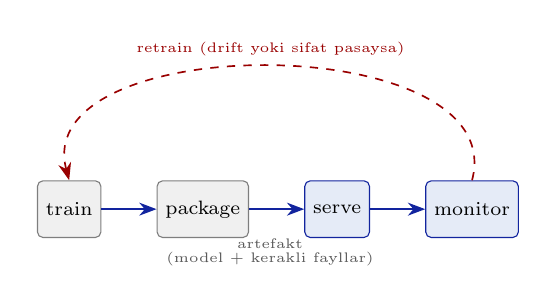
\begin{tikzpicture}[node distance=0.7cm]
    \node[flowonce] (tr) {train};
    \node[flowonce, right=of tr] (pk) {package};
    \node[flowbox,  right=of pk] (sv) {serve};
    \node[flowbox,  right=of sv] (mo) {monitor};

    \draw[flowarr] (tr)--(pk);
    \draw[flowarr] (pk)--(sv);
    \draw[flowarr] (sv)--(mo);

    \node[font=\tiny, gray!70!black, align=center]
      at ($(pk)!0.5!(sv)+(0,-0.55)$) {artefakt\\[-1pt](model + kerakli fayllar)};

    \draw[backarr] (mo.north) to[out=75,in=105]
      node[above, font=\tiny, deepred]{retrain (drift yoki sifat pasaysa)} (tr.north);
  \end{tikzpicture}\\[2pt]

  {\scriptsize\color{gray!70!black}
   kulrang $=$ davriy / zaruratga ko\uzq{}ra \qquad
   {\color{cnublue}ko\uzq{}k $=$ xizmat ishlayotgan bosqichlar}}
  \end{center}

  \vspace{1pt}

  \footnotesize
  \textbf{Mazmuni:}
  \textit{train} --- modelni o\uzq{}qitish;
  \textit{package} --- model artefakti, bog\uzq{}liqliklar va kerakli fayllarni tayyorlash;
  \textit{serve} --- modelni API orqali ishlatish;
  \textit{monitor} --- sifat, kechikish va xatolarni kuzatish;
  \textit{retrain} --- kerak bo\uzq{}lsa modelni qayta o\uzq{}qitish.
\end{frame}

% ----------------------------------------------------------------
% [H1] KELTIRIB CHIQARISH
% ----------------------------------------------------------------
\begin{frame}{Asoslash: nega bosqichlarni ajratamiz?}
  \small

  \begin{columns}[T,totalwidth=\textwidth]
    \begin{column}{0.58\textwidth}
      \begin{enumerate}\setlength\itemsep{5pt}
        \item \textbf{O\uzq{}qitish qimmat.}
        Modelni har bir so\uzq{}rovda qayta o\uzq{}qitib bo\uzq{}lmaydi.

        \item \textbf{Model artefaktga aylantiriladi.}
        O\uzq{}qitilgan model, tokenizer/preprocessing va sozlamalar saqlanadi.

        \item \textbf{Xizmat bosqichi tez ishlashi kerak.}
        Server ishga tushganda artefaktni yuklaydi; har so\uzq{}rovda esa faqat
        bashorat (\textit{inference}) bajariladi.

        \item \textbf{Monitoring siklni yopadi.}
        Sifat, kechikish va xatolar kuzatiladi; muammo aniqlansa, model qayta
        o\uzq{}qitiladi yoki yangi versiya chiqariladi.
      \end{enumerate}
    \end{column}

    \begin{column}{0.39\textwidth}
      \begin{tcolorbox}[defbox,top=2pt,bottom=2pt]
        \footnotesize
        \centering
        \textbf{Ajratilgan oqim}\\[3pt]
        \textit{train}
        $\rightarrow$
        \textit{artifact}
        $\rightarrow$
        \textit{serve}\\[2pt]
        $\rightarrow$
        \textit{monitor}
        $\rightarrow$
        \textit{retrain}
      \end{tcolorbox}

      \vspace{4pt}

      \begin{tcolorbox}[okbox,top=2pt,bottom=2pt]
        \footnotesize
        \textbf{Xulosa:}
        bosqichlarni ajratish xizmatni tezroq, takrorlanuvchanroq va
        boshqariladigan qiladi.
      \end{tcolorbox}
    \end{column}
  \end{columns}
\end{frame}

% ----------------------------------------------------------------
% [I1] QO\uzq{}LDA MISOL (ILLYUSTRATIV --- locked emas)
% ----------------------------------------------------------------
\begin{frame}[t]{Qo\uzq{}lda misol: modelni bir marta yuklash}
  \small
  \vspace{-2mm}

  \begin{tcolorbox}[defbox, boxsep=1pt, left=4pt, right=4pt, top=2pt, bottom=2pt]
    \footnotesize
    \textbf{Sharoit:} model fayli $400$ MB; yuklash vaqti $\approx 2$ s,
    bitta bashorat vaqti $\approx 20$ ms.
  \end{tcolorbox}

  \vspace{2pt}

  \begin{columns}[T,totalwidth=\textwidth]
    \begin{column}{0.48\textwidth}
      \footnotesize

      \textbf{1) Har so\uzq{}rovda yuklash:}\\
      $2000 + 20 = 2020$ ms/so\uzq{}rov
      $= 2.02$ s/so\uzq{}rov. Bu juda sekin.\\[4pt]

      \textbf{2) Server startida bir marta yuklash:}\\
      barqaror ish rejimida har so\uzq{}rov $\approx 20$ ms.\\[4pt]

      \textbf{Taqqoslash:}\\
      $\dfrac{2020}{20}=101 \Rightarrow$
      amalda \textbf{taxminan $100\times$ tezroq}.

      \vspace{4pt}

      \begin{tcolorbox}[okbox, top=2pt, bottom=2pt, left=3pt, right=3pt]
        \scriptsize
        Model server ishga tushganda \textbf{xotiraga bir marta yuklanadi};
        keyingi so\uzq{}rovlar shu nusxadan foydalanadi.
        \textbf{Eslatma:} yuklash server startini sekinlashtiradi;
        agar lazy loading ishlatilsa, birinchi so\uzq{}rov ham sekin bo\uzq{}lishi mumkin.
      \end{tcolorbox}
    \end{column}

    \begin{column}{0.52\textwidth}
  \centering
  {\footnotesize\textbf{Bitta so\uzq{}rov uchun kechikish}}\\[2pt]

  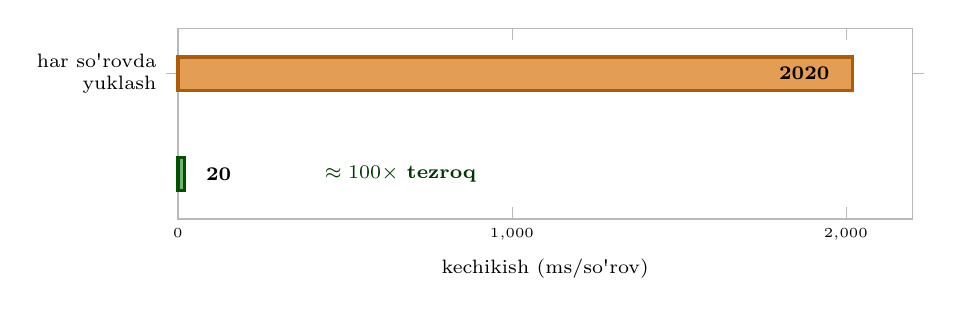
\begin{tikzpicture}
    \begin{axis}[
      intuit,
      width=0.90\linewidth,
      height=4.0cm,
      xbar,
      bar width=12pt,
      xmin=0,
      xmax=2200,
      ytick=data,
      symbolic y coords={startda,har_sorovda},
      yticklabels={
        {\shortstack[r]{har so\uzq{}rovda\\yuklash}},
        {\shortstack[r]{har so\uzq{}rovda\\yuklash}}
      },
      yticklabel style={font=\scriptsize, align=right},
      xlabel={kechikish (ms/so\uzq{}rov)},
      xtick={0,1000,2000},
      enlarge y limits=0.45,
      clip=false,
      every axis plot/.append style={bar shift=0pt}
    ]
      \addplot[draw=cwarn!80!black, fill=cwarn!70]
        coordinates {(2020,har_sorovda)};
      \node[black, font=\scriptsize\bfseries, anchor=east]
        at (axis cs:1980,har_sorovda) {2020};

      \addplot[draw=deepgreen!70!black, fill=deepgreen!55]
        coordinates {(20,startda)};
      \node[black, font=\scriptsize\bfseries, anchor=west]
        at (axis cs:55,startda) {20};

      \node[deepgreen!50!black, font=\scriptsize\bfseries, anchor=west]
        at (axis cs:410,startda) {$\approx 100\times$ tezroq};
    \end{axis}
  \end{tikzpicture}
\end{column}
\end{columns}
\end{frame}
% ----------------------------------------------------------------
% [J1] SIZNING VAZIFANGIZ
% ----------------------------------------------------------------
\begin{frame}{Sizning vazifangiz: soniyadagi yukni hisoblash}
  \small

  \begin{tcolorbox}[warnbox,title=Savol,top=2pt,bottom=2pt]
    Server ishga tushganda model xotiraga bir marta yuklangan.
    Har bir bashorat $\approx 20$ ms davom etadi.
    Bitta jarayon ketma-ket ishlasa, server bir soniyada taxminan
    nechta so\uzq{}rovga javob bera oladi?
  \end{tcolorbox}

  \pause

  \vspace{3pt}

  \begin{tcolorbox}[okbox,title=Javob,top=2pt,bottom=2pt]
    \[
      \text{so\uzq{}rov/soniya}
      \approx
      \frac{1000\ \text{ms}}{20\ \text{ms}}
      =
      \mathbf{50}
    \]

    \footnotesize
    Demak, bitta jarayon ketma-ket ishlaganda nazariy maksimum
    $\approx 50$ so\uzq{}rov/soniya. Amalda API, tarmoq va navbat
    (\textit{queue}) xarajatlari sababli qiymat biroz past bo\uzq{}lishi mumkin.\\[3pt]

    Ko\uzq{}proq yuk kerak bo\uzq{}lsa, bir nechta \textbf{worker/replica}
    ishga tushiriladi yoki mos holatda so\uzq{}rovlar \textbf{batch}
    qilib qayta ishlanadi. Bu --- \textbf{masshtablash}.
  \end{tcolorbox}
\end{frame}

% ----------------------------------------------------------------
% [K1] KOD <-> FORMULA  [fragile]
% ----------------------------------------------------------------
\begin{frame}[fragile]{Kod $\leftrightarrow$ jarayon: modelni bir marta yuklash}
  \small

  \begin{columns}[T,totalwidth=\textwidth]
    \begin{column}{0.59\textwidth}
\begin{lstlisting}[basicstyle=\ttfamily\scriptsize]
# server startida BIR MARTA
clf = FineTunedClassifier()
clf.load("m13_model")     # artefaktni yuklash

# har so'rovda: faqat inference
def predict(text):
    return clf.predict(text)
\end{lstlisting}
    \end{column}

    \begin{column}{0.38\textwidth}
      \textbf{Kod $\to$ MLOps ma'nosi}\\[3pt]

      \footnotesize
      \renewcommand{\arraystretch}{1.12}
      \begin{tabular}{p{1.7cm}p{2.35cm}}
        \toprule
        \textbf{Kod} & \textbf{Vazifa} \\
        \midrule
        \texttt{load} &
        serve startida artefaktni xotiraga yuklash \\
        \texttt{predict} &
        har so\uzq{}rovda bashorat qilish \\
        \bottomrule
      \end{tabular}

      \vspace{5pt}

      \begin{tcolorbox}[okbox,top=2pt,bottom=2pt,left=3pt,right=3pt]
        \footnotesize
        \textbf{G\uzq{}oya:}
        \texttt{load} bir marta bajariladi;
        \texttt{predict} esa har so\uzq{}rovda ishlaydi.
        Shuning uchun so\uzq{}rov vaqti asosan \textit{inference} vaqtiga teng.
      \end{tcolorbox}
    \end{column}
  \end{columns}
\end{frame}

% ----------------------------------------------------------------
% [L1] TUZOG\uzq{}
% ----------------------------------------------------------------
\begin{frame}{Deploy tuzog\uzq{}i: train--serve tafovuti}
  \small

  \begin{columns}[T,totalwidth=\textwidth]
    \begin{column}{0.51\textwidth}
      \begin{tcolorbox}[warnbox,title={Muammo: training-serving skew},top=2pt,bottom=2pt]
        \footnotesize
        Train paytida ishlatilgan \textbf{preprocessing} xizmatda aynan
        takrorlanmasa, model boshqa ko\uzq{}rinishdagi kirishni ko\uzq{}radi.\\[3pt]

        \textbf{Misol:} tokenizer, normalizatsiya yoki TF--IDF/vectorizer
        versiyasi mos kelmasa, bashorat ishonchsiz bo\uzq{}ladi.
      \end{tcolorbox}

      \vspace{4pt}

      \begin{tcolorbox}[defbox,top=2pt,bottom=2pt]
        \scriptsize
        \textbf{Intuitsiya:} model xom matnni emas, train paytida hosil qilingan
        aynan shu \textbf{xususiyatlar ko\uzq{}rinishi}ni o\uzq{}rgangan.
      \end{tcolorbox}
    \end{column}

    \begin{column}{0.46\textwidth}
      \begin{tcolorbox}[okbox,title={Yechim},top=2pt,bottom=2pt]
        \footnotesize
        \begin{enumerate}\setlength\itemsep{2pt}
          \item Bir xil preprocessing modulidan foydalanish.
          \item Tokenizer/vectorizer va konfiguratsiyani model bilan birga
                saqlash.
          \item Model, kod va preprocessing versiyasini birga belgilash.
          \item Train va serve chiqishini solishtiruvchi oddiy test yozish.
        \end{enumerate}
      \end{tcolorbox}

      \vspace{4pt}

      \begin{tcolorbox}[okbox,top=2pt,bottom=2pt]
        \scriptsize
        \textbf{Amaliy qoida:}
        model artefakti yolg\uzq{}iz saqlanmaydi; u tokenizer,
        preprocessing kodi va versiya ma\uzq{}lumotlari bilan birga yuradi.
      \end{tcolorbox}
    \end{column}
  \end{columns}
\end{frame}

% ================================================================
\section[API va Docker]{API yaratish va Docker bilan konteynerlashtirish}
% ================================================================

% ----------------------------------------------------------------
% [F2] INTUITSIYA
% ----------------------------------------------------------------
\begin{frame}{Intuitsiya: modelga kirish nuqtasi va barqaror muhit}
  \small
\vspace{-4mm}
  \begin{columns}[T,totalwidth=\textwidth]
    \begin{column}{0.50\textwidth}
      \begin{tcolorbox}[defbox,top=2pt,bottom=2pt,left=4pt,right=4pt]
        \footnotesize
        \textbf{API} (\textit{Application Programming Interface}) ---
        modelga tashqi tizimlar murojaat qiladigan standart
        \textbf{kirish nuqtasi}.\\[2pt]

        Masalan, boshqa dastur HTTP/JSON so\uzq{}rov yuboradi va modeldan
        bashorat javobini oladi.
      \end{tcolorbox}

      \vspace{-2pt}

      \begin{tcolorbox}[defbox,top=2pt,bottom=2pt,left=4pt,right=4pt]
        \footnotesize
        \textbf{Docker} --- modelni ishga tushirish muhitini
        barqarorlashtirish usuli.\\[2pt]

        Kod, kutubxonalar va model fayllari bir xil muhitda ishlashi uchun
        konteynerdan foydalaniladi.
      \end{tcolorbox}

      \vspace{-2pt}

      \begin{tcolorbox}[okbox,top=2pt,bottom=2pt,left=4pt,right=4pt]
        \scriptsize
        \textbf{Kalit fikr:}
        FastAPI modelga kirish nuqtasini beradi; Docker esa xizmatni
        boshqa serverda qayta ishga tushirishni osonlashtiradi.
      \end{tcolorbox}
    \end{column}

    \begin{column}{0.47\textwidth}
      \begin{tcolorbox}[okbox,title={Minimal xizmat oqimi},top=2pt,bottom=2pt,left=4pt,right=4pt]
        \centering
        \scriptsize
        \textbf{Foydalanuvchi / dastur}\\
        {\tiny HTTP/JSON so\uzq{}rov}\\[-1pt]
        $\Downarrow$\\[-1pt]
        \textbf{FastAPI endpoint}\\
        {\tiny \texttt{POST /predict}}\\[-1pt]
        $\Downarrow$\\[-1pt]
        \textbf{NLP model}\\
        {\tiny bashorat / inference}\\[-1pt]
        $\Downarrow$\\[-1pt]
        \textbf{JSON javob}
      \end{tcolorbox}

      \vspace{5pt}

      \begin{tcolorbox}[defbox,top=2pt,bottom=2pt,left=4pt,right=4pt]
        \footnotesize
        \textbf{Bu slayddagi savol:}
        foydalanuvchi modelga qanday murojaat qiladi va xizmat boshqa
        muhitda qanday barqaror ishlaydi?
      \end{tcolorbox}
    \end{column}
  \end{columns}
\end{frame}

% ----------------------------------------------------------------
% [G2] RASMIY TA\uzq{}RIF + BUNDA
% ----------------------------------------------------------------
\begin{frame}{API va konteyner: rasmiy ta\uzq{}rif}
  \small

  \begin{tcolorbox}[defbox,top=2pt,bottom=2pt,left=4pt,right=4pt]
    \centering
    \textbf{API:}\quad
    \textit{request} $\rightarrow$ \textit{response}
    \hspace{1.2em}
    \textbf{Docker image:}\quad
    \textit{base image} $+$ \textit{deps} $+$ \textit{model} $+$ \textit{kod}
    \hspace{1.2em}
    \textbf{Container:}\quad
    \textit{ishga tushgan image}
  \end{tcolorbox}

  \vspace{3pt}

  \begin{columns}[T,totalwidth=\textwidth]
    \begin{column}{0.50\textwidth}
      \footnotesize
      \textbf{API} --- HTTP endpoint orqali modelga murojaat qilish usuli.
      Masalan: \texttt{POST /predict}.\\[4pt]

      \textbf{Image} --- Docker tasviri: bazaviy muhit(base image), kutubxonalar(deps),
      model fayllari va ilova kodining paketlangan ko\uzq{}rinishi.\\[4pt]

      \textbf{Container} --- image ning \textbf{ishga tushgan nusxasi}.
      Ya\uzq{}ni image tayyor shablon bo\uzq{}lsa, container shu shablon asosida
      ishlayotgan jarayondir.\\[5pt]

      \begin{tcolorbox}[okbox,top=2pt,bottom=2pt,left=3pt,right=3pt]
        \scriptsize
        \textbf{Kalit farq:}
        image quriladi va saqlanadi; container esa shu image asosida ishga
        tushiriladi.
      \end{tcolorbox}
    \end{column}

    \begin{column}{0.47\textwidth}
      \centering
      \vspace{-9pt}
      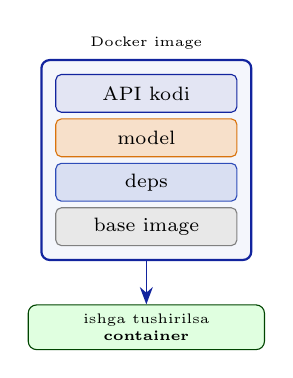
\begin{tikzpicture}[every node/.style={font=\scriptsize}, node distance=2pt]
        \node[flowbox, fill=gray!18, draw=black!50,
              minimum width=2.3cm, minimum height=0.48cm] (l1) {base image};

        \node[flowbox, fill=cdeps!18, draw=cdeps,
              minimum width=2.3cm, minimum height=0.48cm, above=of l1] (l2) {deps};

        \node[flowbox, fill=cmodel!22, draw=cmodel,
              minimum width=2.3cm, minimum height=0.48cm, above=of l2] (l3) {model};

        \node[flowbox, fill=cnublue!12, draw=cnublue,
              minimum width=2.3cm, minimum height=0.48cm, above=of l3] (l4) {API kodi};

        \begin{scope}[on background layer]
          \node[
            draw=cnublue, thick, rounded corners=3pt, fill=cnubluebg!45,
            fit=(l1)(l4), inner sep=5pt,
            label={[font=\tiny]above:Docker image}
          ] (img) {};
        \end{scope}

        \node[
          draw=deepgreen!60!black, fill=green!12, rounded corners=3pt,
          below=0.55cm of img, minimum width=3.0cm, minimum height=0.55cm,
          font=\tiny, align=center
        ] (cont) {ishga tushirilsa\\\textbf{container}};

        \draw[flowarr] (img.south) -- (cont.north);
      \end{tikzpicture}

      \vspace{-3pt}

      \begin{tcolorbox}[defbox,top=2pt,bottom=2pt,left=4pt,right=4pt]
        \scriptsize
        \textbf{Eslatma:}
        Docker takrorlanuvchan ishga tushirishni osonlashtiradi, lekin
        apparat, GPU drayveri va tashqi servislar ham muhim.
      \end{tcolorbox}
    \end{column}
  \end{columns}
\end{frame}


% ----------------------------------------------------------------
% [G2b] FASTAPI ENDPOINT (qo\uzq{}shimcha amaliy ko\uzq{}prik)
% ----------------------------------------------------------------
\begin{frame}[fragile]{Kod $\leftrightarrow$ xizmat: minimal FastAPI endpoint}
  \small

  \begin{columns}[T,totalwidth=\textwidth]
    \begin{column}{0.59\textwidth}
\begin{lstlisting}[basicstyle=\ttfamily\scriptsize]
from fastapi import FastAPI
from pydantic import BaseModel

class PredictRequest(BaseModel):
    text: str

app = FastAPI()
model = load_model("model/")   # server startida bir marta

@app.post("/predict")
def predict(req: PredictRequest):
    pred = model.predict(req.text)
    return {
        "label": pred.label,
        "confidence": pred.score
    }
\end{lstlisting}
    \end{column}

    \begin{column}{0.38\textwidth}
      \textbf{Kod $\to$ MLOps ma\uzq{}nosi}\\[3pt]

      \footnotesize
      \renewcommand{\arraystretch}{1.12}
      \begin{tabular}{p{1.75cm}p{2.05cm}}
        \toprule
        \textbf{Kod} & \textbf{Vazifa} \\
        \midrule
        \texttt{BaseModel} & kirish sxemasi \\
        \texttt{/predict} & HTTP endpoint \\
        \texttt{load\_model} & artefaktni yuklash \\
        \texttt{return} & JSON javob \\
        \bottomrule
      \end{tabular}

      \vspace{5pt}

      \begin{tcolorbox}[okbox,top=2pt,bottom=2pt,left=3pt,right=3pt]
        \footnotesize
        API matnni JSON so\uzq{}rov orqali qabul qiladi va model bashoratini
        JSON javob sifatida qaytaradi. Shu sababli model boshqa dasturlar
        bilan ulanishi mumkin.
      \end{tcolorbox}
    \end{column}
  \end{columns}
\end{frame}

% ----------------------------------------------------------------
% [H2] KELTIRIB CHIQARISH
% ----------------------------------------------------------------
\begin{frame}{Asoslash: nega Docker kerak?}
  \small

  \begin{columns}[T,totalwidth=\textwidth]
    \begin{column}{0.52\textwidth}
      \begin{tcolorbox}[warnbox,title={Muammo},top=2pt,bottom=2pt]
        \footnotesize
        Model kutubxona va versiyalarga bog\uzq{}liq:
        \texttt{torch}, \texttt{scikit-learn}, tokenizer, config va boshqa fayllar.\\[3pt]

        Agar train muhiti va server muhiti farq qilsa, model ishlamasligi
        yoki natija takrorlanmasligi mumkin.
      \end{tcolorbox}

      \vspace{4pt}

      \begin{tcolorbox}[defbox,top=2pt,bottom=2pt]
        \footnotesize
        \textbf{Docker image} odatda quyidagilarni bir joyga yig\uzq{}adi:\\[2pt]
        \centering
        \textit{base image} $+$ \textit{deps} $+$ \textit{kod} $+$ \textit{model}
      \end{tcolorbox}
    \end{column}

    \begin{column}{0.45\textwidth}
      \begin{tcolorbox}[okbox,title={Docker nima beradi?},top=2pt,bottom=2pt]
        \footnotesize
        \begin{enumerate}\setlength\itemsep{2pt}
          \item Kutubxonalar va ishga tushirish muhitini aniqroq belgilaydi.
          \item Ilova kodi, model fayllari va sozlamalarni bitta birlikka yig\uzq{}adi.
          \item Shu image turli serverlarda o\uzq{}xshash muhitda ishga tushadi.
        \end{enumerate}
      \end{tcolorbox}

      \vspace{4pt}

      \begin{tcolorbox}[okbox,top=2pt,bottom=2pt]
        \footnotesize
        \textbf{Xulosa:}
        API modelga kirish nuqtasini beradi; Docker esa xizmatni
        barqaror va takrorlanuvchan muhitda ishga tushirishga yordam beradi.
      \end{tcolorbox}
    \end{column}
  \end{columns}
\end{frame}

% ----------------------------------------------------------------
% [I2] QO\uzq{}LDA MISOL (ILLYUSTRATIV)
% ----------------------------------------------------------------
\begin{frame}{Qo\uzq{}lda misol: Docker image qatlamlari}
  \small

  \begin{tcolorbox}[defbox]
    \footnotesize
    \textbf{Soddalashtirilgan misol:}
    \textit{base image} ($\approx 120$ MB)
    $+$ \textit{kutubxonalar} ($\approx 800$ MB)
    $+$ \textit{model} ($\approx 400$ MB)
    $+$ \textit{kod} ($\approx 10$ MB).
  \end{tcolorbox}

  \vspace{2pt}

  \begin{columns}[T,totalwidth=\textwidth]
    \begin{column}{0.55\textwidth}
      \footnotesize

      Jami image hajmi $\approx 1330$ MB. Docker image bir nechta
      \textbf{qatlam}lardan tuziladi.\\[4pt]

      Agar \texttt{requirements.txt} o\uzq{}zgarmasa, kutubxonalar qatlami
      odatda \textbf{keshdan olinadi}. Agar faqat kod o\uzq{}zgarsa,
      pastdagi qatlamlar saqlanib qoladi, \textbf{o\uzq{}zgargan qatlam va undan
      keyingilar} qayta quriladi.\\[5pt]

      \begin{tcolorbox}[okbox,top=2pt,bottom=2pt,left=3pt,right=3pt]
        \footnotesize
        \textbf{Amaliy qoida:}
        avval \texttt{requirements.txt} ni nusxalab kutubxonalarni
        o\uzq{}rnating, \textbf{kodni esa oxirida} nusxalang.
        Shunda kod tez-tez o\uzq{}zgarganda kesh samaraliroq ishlaydi.
      \end{tcolorbox}
    \end{column}

    \begin{column}{0.42\textwidth}
      \centering
      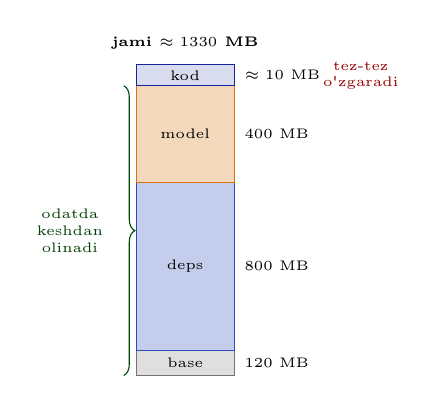
\begin{tikzpicture}[every node/.style={font=\tiny}]
        \def\w{1.25cm}

        % base
        \fill[gray!25, draw=black!55] (0,0.00) rectangle (\w,0.32);
        \node at (0.62,0.16) {base};
        \node[right] at (\w,0.16) {120 MB};

        % deps
        \fill[cdeps!28, draw=cdeps] (0,0.32) rectangle (\w,2.45);
        \node at (0.62,1.39) {deps};
        \node[right] at (\w,1.39) {800 MB};

        % model
        \fill[cmodel!28, draw=cmodel] (0,2.45) rectangle (\w,3.68);
        \node at (0.62,3.07) {model};
        \node[right] at (\w,3.07) {400 MB};

        % code
        \fill[cnublue!16, draw=cnublue] (0,3.68) rectangle (\w,3.95);
        \node at (0.62,3.81) {kod};
        \node[right] at (\w,3.81) {$\approx 10$ MB};

        \node[font=\tiny\bfseries, above=2pt] at (0.62,3.95) {jami $\approx 1330$ MB};

        % brace for cached layers when only code changes
        \draw[decorate, decoration={brace, amplitude=4pt}, deepgreen!60!black]
          (-0.16,3.68) -- (-0.16,0)
          node[midway, left=4pt, deepgreen!55!black, font=\tiny, align=center]
          {odatda\\keshdan\\olinadi};

        \node[font=\tiny, deepred, align=center] at (2.85,3.81)
          {tez-tez\\o\uzq{}zgaradi};
      \end{tikzpicture}
    \end{column}
  \end{columns}
\end{frame}

% ----------------------------------------------------------------
% [J2] SIZNING VAZIFANGIZ
% ----------------------------------------------------------------
\begin{frame}{Sizning vazifangiz: faqat kod o\uzq{}zgardi}
  \small

  \begin{tcolorbox}[warnbox,title=Savol,top=2pt,bottom=2pt]
    Siz faqat ilova kodini o\uzq{}zgartirdingiz.
    Kutubxonalar va model fayllari o\uzq{}zgarmadi.
    Qaysi qatlamlar keshdan olinadi, qaysi qatlam qayta quriladi?
  \end{tcolorbox}

  \pause

  \vspace{3pt}

  \begin{tcolorbox}[okbox,title=Javob,top=2pt,bottom=2pt]
    Agar Dockerfile tartibi
    \[
      \text{base} \rightarrow \text{deps} \rightarrow \text{model} \rightarrow \text{kod}
    \]
    bo\uzq{}lsa, \textbf{base}, \textbf{deps} va \textbf{model} qatlamlari
    keshdan olinadi; faqat \textbf{kod} qatlami qayta quriladi.\\[3pt]

    \footnotesize
    \textbf{Qoida:} Docker’da o\uzq{}zgargan qatlam va undan keyingi qatlamlar
    qayta quriladi. Shuning uchun kam o\uzq{}zgaradigan narsalar
    yuqoriroqqa, tez o\uzq{}zgaradigan kod esa pastroqqa qo\uzq{}yiladi.
  \end{tcolorbox}
\end{frame}

% ----------------------------------------------------------------
% [K2] KOD <-> FORMULA  [fragile]
% ----------------------------------------------------------------
\begin{frame}[fragile]{Kod $\leftrightarrow$ bosqich: Dockerfile}
  \small

  \begin{columns}[T,totalwidth=\textwidth]
    \begin{column}{0.59\textwidth}
\begin{lstlisting}[basicstyle=\ttfamily\scriptsize]
FROM python:3.11-slim          # base image

WORKDIR /app

COPY requirements.txt .
RUN pip install --no-cache-dir -r requirements.txt  # deps

COPY model/ ./model/           # model artefakti
COPY app.py ./                 # tez o'zgaradigan kod

EXPOSE 8000
CMD ["uvicorn", "app:app",
     "--host", "0.0.0.0", "--port", "8000"]
\end{lstlisting}
    \end{column}

    \begin{column}{0.38\textwidth}
      \textbf{Qator $\to$ qatlam}\\[3pt]

      \footnotesize
      \renewcommand{\arraystretch}{1.12}
      \begin{tabular}{p{1.75cm}p{2.05cm}}
        \toprule
        \textbf{Qator} & \textbf{Vazifa} \\
        \midrule
        \texttt{FROM} & bazaviy muhit \\
        \texttt{RUN pip} & kutubxonalar \\
        \texttt{COPY model} & model artefakti \\
        \texttt{COPY app} & ilova kodi \\
        \texttt{CMD} & ishga tushirish \\
        \bottomrule
      \end{tabular}

      \vspace{5pt}

      \begin{tcolorbox}[okbox,top=2pt,bottom=2pt,left=3pt,right=3pt]
        \footnotesize
        \textbf{Kesh g\uzq{}oyasi:}
        kam o\uzq{}zgaradigan qatlamlar yuqorida, tez o\uzq{}zgaradigan
        \texttt{app.py} pastda turadi. Shunda faqat kod o\uzq{}zgarsa,
        base, deps va model qatlamlari keshdan olinadi.
      \end{tcolorbox}
    \end{column}
  \end{columns}
\end{frame}

% ----------------------------------------------------------------
% [L2] TUZOG\uzq{}
% ----------------------------------------------------------------
\begin{frame}{Docker tuzog\uzq{}i: katta image va maxfiy kalitlar}
  \small

  \begin{columns}[T,totalwidth=\textwidth]
    \begin{column}{0.51\textwidth}
      \begin{tcolorbox}[warnbox,title={Muammo},top=2pt,bottom=2pt]
        \footnotesize
        Keraksiz fayllar --- datasetlar, cache, notebooklar va loglar ---
        image hajmini kattalashtiradi.\\[3pt]

        API kaliti, token yoki parolni image ichiga yozish esa
        \textbf{xavfsizlik xatosi}: image tarqalsa, maxfiy ma\uzq{}lumot ham
        tarqaladi.
      \end{tcolorbox}
    \end{column}

    \begin{column}{0.46\textwidth}
      \begin{tcolorbox}[okbox,title={Yechim},top=2pt,bottom=2pt]
        \footnotesize
        \begin{enumerate}\setlength\itemsep{2pt}
          \item \texttt{.dockerignore} bilan keraksiz fayllarni image ga kiritmang.
          \item \texttt{python:3.11-slim} kabi yengil base image ishlating.
          \item Maxfiy kalitlarni kod yoki image ichiga yozmang.
          \item Lokal ishda environment o\uzq{}zgaruvchilari, production da esa
                secrets manager ishlating.
        \end{enumerate}
      \end{tcolorbox}
    \end{column}
  \end{columns}

  \vspace{4pt}

  \begin{tcolorbox}[defbox,top=2pt,bottom=2pt,left=4pt,right=4pt]
    \footnotesize
    \textbf{Eslatma:} Docker muhitni takrorlashni osonlashtiradi, lekin
    \textbf{mutlaq bir xil natijani kafolatlamaydi}. CPU arxitekturasi
    (x86/ARM), GPU drayveri, CUDA versiyasi yoki tashqi servislar farq qilsa,
    ishlash tezligi va ba'zan natija ham farq qilishi mumkin.
  \end{tcolorbox}
\end{frame}

% ================================================================
\section[Monitoring]{Model monitoringi va versiyalash}
% ================================================================

% ----------------------------------------------------------------
% [F3] INTUITSIYA
% ----------------------------------------------------------------
\begin{frame}{Intuitsiya: model eskiradi, uni kuzatib borish kerak}
  \small

  \begin{columns}[T,totalwidth=\textwidth]
    \begin{column}{0.52\textwidth}
      \begin{tcolorbox}[warnbox,title={Nega monitoring kerak?},top=2pt,bottom=2pt]
        \footnotesize
        Foydalanuvchi matnlari vaqt o\uzq{}tishi bilan o\uzq{}zgaradi:
        yangi so\uzq{}zlar, yangi mavzular, yangi yozish uslublari paydo bo\uzq{}ladi.\\[3pt]

        Model esa avvalgi ma\uzq{}lumot taqsimotida o\uzq{}qitilgan.
        Shuning uchun ma\uzq{}lumot siljishi (\textit{drift}) yuz bersa,
        model sifati pasayishi mumkin.
      \end{tcolorbox}

      \vspace{4pt}

      \begin{tcolorbox}[okbox,top=2pt,bottom=2pt]
        \footnotesize
        \textbf{Yechim:}
        metrikalarni kuzatish, muammo bo\uzq{}lsa ogohlantirish,
        kerak bo\uzq{}lsa yangi model versiyasiga o\uzq{}tish.
      \end{tcolorbox}
    \end{column}

    \begin{column}{0.45\textwidth}
      \begin{tcolorbox}[defbox,title={Monitoring oqimi},top=2pt,bottom=2pt]
        \centering
        \footnotesize
        \textbf{kuzatish}\\[-1pt]
        {\scriptsize latency, xatolar, sifat metrikalari}\\[2pt]
        $\Downarrow$\\[-1pt]
        \textbf{ogohlantirish}\\[-1pt]
        {\scriptsize threshold buzilsa}\\[2pt]
        $\Downarrow$\\[-1pt]
        \textbf{versiyalash / rollback}\\[-1pt]
        {\scriptsize yangi model yoki eski barqaror versiya}
      \end{tcolorbox}

      \vspace{4pt}

      \begin{tcolorbox}[okbox,top=2pt,bottom=2pt]
        \footnotesize
        \textbf{Model reyestri} (\textit{model registry}) v1, v2, \dots
        versiyalarni, metrikalarni va kerakli fayllarni saqlaydi.
        Xato bo\uzq{}lsa, eski barqaror versiyaga qaytish
        (\textit{rollback}) mumkin.
      \end{tcolorbox}
    \end{column}
  \end{columns}
\end{frame}

% ----------------------------------------------------------------
% [G3] RASMIY TA\uzq{}RIF + BUNDA
% ----------------------------------------------------------------
\begin{frame}{Monitoring va drift: rasmiy ta\uzq{}rif}
  \small

  \begin{tcolorbox}[defbox]
    \centering
    \textbf{Oddiy ogohlantirish qoidasi:}\qquad
    $\Delta = M_{\text{base}} - M_{\text{joriy}}, \qquad
    \Delta \ge \tau \Rightarrow \text{ogohlantirish}$
  \end{tcolorbox}

  \vspace{2pt}

  \begin{columns}[T,totalwidth=\textwidth]
    \begin{column}{0.44\textwidth}
      \footnotesize
      \textbf{Bu yerda:}
      $M_{\text{base}}$ --- boshlang\uzq{}ich metrika,
      $M_{\text{joriy}}$ --- joriy o\uzq{}lchov,
      $\Delta$ --- pasayish,
      $\tau$ --- chegaraviy qiymat.\\[4pt]

      Bu qoida \textbf{F1}, \textbf{accuracy} kabi
      ``katta bo\uzq{}lsa yaxshi'' metrikalar uchun qulay.\\[5pt]

      \begin{tcolorbox}[okbox,top=2pt,bottom=2pt,left=3pt,right=3pt]
        \scriptsize
        Agar $\Delta \ge \tau$ bo\uzq{}lsa, avval \textbf{ogohlantirish} beriladi;
        so\uzq{}ng sabab tekshiriladi va kerak bo\uzq{}lsa
        \textbf{retrain} yoki \textbf{rollback} qilinadi.
      \end{tcolorbox}

      \vspace{3pt}
      {\scriptsize
      \textbf{Eslatma:} yorliqlar bo\uzq{}lmasa, bevosita sifatni emas,
      kiruvchi ma\uzq{}lumotdagi \textit{data drift} indikatorlarini
      (masalan, token taqsimoti, uzunlik, yangi so\uzq{}zlar ulushi) kuzatamiz.
      }
    \end{column}

    \begin{column}{0.53\textwidth}
      \centering
      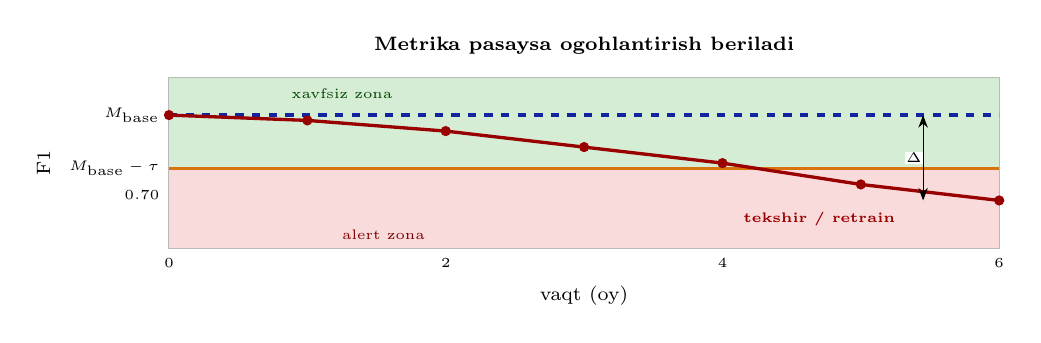
\begin{tikzpicture}
        \begin{axis}[
          intuit,
          height=3.75cm,
          width=\linewidth,
          xlabel={vaqt (oy)},
          ylabel={F1},
          xmin=0, xmax=6,
          ymin=0.60, ymax=0.92,
          xtick={0,2,4,6},
          ytick={0.70,0.75,0.85},
          yticklabels={$0.70$,$M_{\text{base}}-\tau$,$M_{\text{base}}$},
          title={Metrika pasaysa ogohlantirish beriladi}
        ]
          % xavfsiz va alert hududlari
          \fill[cokfill]    (axis cs:0,0.75) rectangle (axis cs:6,0.92);
          \fill[calertfill] (axis cs:0,0.60) rectangle (axis cs:6,0.75);

          % base va threshold chiziqlari
          \addplot[cnublue, dashed, domain=0:6, samples=2] {0.85};
          \addplot[cwarn,   domain=0:6, samples=2] {0.75};

          % joriy metrika trayektoriyasi
          \addplot[deepred, mark=*, mark size=1.2pt]
            coordinates {(0,0.85)(1,0.84)(2,0.82)(3,0.79)(4,0.76)(5,0.72)(6,0.69)};

          % Delta ko'rsatkichi
          \draw[{Stealth[length=1.6mm]}-{Stealth[length=1.6mm]}, thin, black]
            (axis cs:5.45,0.85) -- (axis cs:5.45,0.69)
            node[midway, left, font=\tiny, fill=white, inner sep=0.4pt] {$\Delta$};

          % yozuvlar
          \node[deepgreen!60!black, font=\tiny] at (axis cs:1.25,0.89) {xavfsiz zona};
          \node[deepred!80!black,   font=\tiny] at (axis cs:1.55,0.625) {alert zona};
          \node[deepred, font=\tiny\bfseries] at (axis cs:4.7,0.655) {tekshir / retrain};
        \end{axis}
      \end{tikzpicture}
    \end{column}
  \end{columns}
\end{frame}

% ----------------------------------------------------------------
% [G3b] MONITORING METRIKALARI: TEXNIK vs MODEL (qo'shilgan)
% ----------------------------------------------------------------
\begin{frame}{Monitoring ikki qatlam: server holati va model sifati}
  \small
\vspace{-3mm}
  \begin{columns}[T,totalwidth=\textwidth]
    \begin{column}{0.49\textwidth}
      \begin{tcolorbox}[defbox,top=2pt,bottom=2pt,left=4pt,right=4pt]
        \footnotesize
        \textbf{1) Texnik monitoring}\\[2pt]
        \scriptsize
        \renewcommand{\arraystretch}{1.08}
        \begin{tabular}{@{}p{2.05cm}p{3.05cm}@{}}
          \toprule
          \textbf{Metrika} & \textbf{Nimani ko\uzq{}rsatadi} \\
          \midrule
          latency & javob kechikishi (ms) \\
          throughput & so\uzq{}rov/soniya \\
          error rate & xato javoblar ulushi \\
          uptime & xizmat mavjudligi \\
          \bottomrule
        \end{tabular}
      \end{tcolorbox}
    \end{column}

    \begin{column}{0.49\textwidth}
      \begin{tcolorbox}[okbox,top=2pt,bottom=2pt,left=4pt,right=4pt]
        \footnotesize
        \textbf{2) Model sifati monitoringi}\\[2pt]
        \scriptsize
        \renewcommand{\arraystretch}{1.08}
        \begin{tabular}{@{}p{2.35cm}p{3.75cm}@{}}
          \toprule
          \textbf{Metrika} & \textbf{Nimani ko\uzq{}rsatadi} \\
          \midrule
          kirish taqsimoti & data drift: $P(X)$ o\uzq{}zgardimi \\
          bashorat taqsimoti & chiqishlar siljidimi \\
          confidence & model ishonchi barqarormi \\
          F1 / accuracy & sifat pasaydimi (yorliq bo\uzq{}lsa) \\
          \bottomrule
        \end{tabular}
      \end{tcolorbox}
    \end{column}
  \end{columns}

  \vspace{6pt}

  \begin{tcolorbox}[warnbox,title={Asosiy farq --- nega ikkalasi kerak?},top=2pt,bottom=2pt,left=4pt,right=4pt]
    \footnotesize
    Server ``yashil'' bo\uzq{}lishi model to\uzq{}g\uzq{}ri ishlayotganini kafolatlamaydi:
    API tez javob berishi mumkin, lekin model noto\uzq{}g\uzq{}ri bashorat qilayotgan
    bo\uzq{}lishi mumkin.\\[2pt]
    \textbf{Data drift:} kirish taqsimoti $P(X)$ o\uzq{}zgaradi, ko\uzq{}pincha
    yorliqsiz kuzatiladi.
    \textbf{Concept drift:} bog\uzq{}liqlik $P(Y|X)$ o\uzq{}zgaradi; odatda
    yorliqli ma\uzq{}lumot va metrika pasayishi orqali tasdiqlanadi.
  \end{tcolorbox}
\end{frame}

% ----------------------------------------------------------------
% [H3] KELTIRIB CHIQARISH
% ----------------------------------------------------------------
\begin{frame}{Asoslash: sifat pasayishini qanday aniqlaymiz?}
  \small
\vspace{-2mm}
  \begin{columns}[T,totalwidth=\textwidth]
    \begin{column}{0.58\textwidth}
      \begin{enumerate}\setlength\itemsep{5pt}
        \item \textbf{Baseline metrikani saqlaymiz.}
        O\uzq{}qitishdan keyin nazorat to\uzq{}plamidagi sifat qayd etiladi:
        $F_{1,\text{base}}$.

        \item \textbf{Joriy metrikani o\uzq{}lchaymiz.}
        Production davrida yangi yorliqlangan namunada sifat hisoblanadi:
        $F_{1,\text{joriy}}$.

        \item \textbf{Pasayishni hisoblaymiz.}
        \[
          \Delta = F_{1,\text{base}} - F_{1,\text{joriy}}
        \]

        \item \textbf{Chegara bilan solishtiramiz.}
        Agar $\Delta \ge \tau$ bo\uzq{}lsa, ogohlantirish beriladi va sabab
        tekshiriladi.
      \end{enumerate}
    \end{column}

    \begin{column}{0.39\textwidth}
      \begin{tcolorbox}[defbox,top=2pt,bottom=2pt,left=4pt,right=4pt]
        \footnotesize
        \textbf{Qaror oqimi:}\\[3pt]
        \centering
        $F_{1,\text{base}}$ va $F_{1,\text{joriy}}$ ni solishtiramiz\\[3pt]
        $\Downarrow$\\[-1pt]
        $\Delta = F_{1,\text{base}} - F_{1,\text{joriy}}$\\[3pt]
        $\Downarrow$\\[-1pt]
        $\Delta \ge \tau$ bo\uzq{}lsa: \textbf{alert}\\[3pt]
        $\Downarrow$\\[-1pt]
        sababni tekshirish $\rightarrow$ retrain yoki rollback
      \end{tcolorbox}

      \vspace{-5pt}

      \begin{tcolorbox}[okbox,top=2pt,bottom=2pt,left=4pt,right=4pt]
        \footnotesize
        \textbf{Xulosa:}
        monitoring sifatning sezilmay pasayishini erta ko\uzq{}rsatadi.
        Bu darhol retrain degani emas; avval sabab aniqlanadi.
      \end{tcolorbox}
    \end{column}
  \end{columns}

  \vspace{2pt}
  {\scriptsize
  \textbf{Eslatma:} bu qoida F1/accuracy kabi ``katta bo\uzq{}lsa yaxshi''
  metrikalar uchun qulay. Yorliqlar bo\uzq{}lmasa, bevosita sifat emas,
  data drift indikatorlari alohida kuzatiladi.
  }
\end{frame}

% ----------------------------------------------------------------
% [I3] QO\uzq{}LDA MISOL (ILLYUSTRATIV)
% ----------------------------------------------------------------
\begin{frame}{Qo\uzq{}lda misol: monitoring chegarasi}
  \small

  \begin{tcolorbox}[defbox,top=2pt,bottom=2pt,left=4pt,right=4pt]
    \footnotesize
    \textbf{Berilgan:}
    baseline $F_{1,\text{base}} = 0.85$;
    bir oydan keyin $F_{1,\text{joriy}} = 0.70$;
    chegara $\tau = 0.10$.
  \end{tcolorbox}

  \vspace{2pt}

  \begin{columns}[T,totalwidth=\textwidth]
    \begin{column}{0.50\textwidth}
      \textbf{Hisob:}

      \begin{align*}
        \Delta &= F_{1,\text{base}} - F_{1,\text{joriy}}\\
               &= 0.85 - 0.70 = 0.15\\
        \Delta &= 0.15 > 0.10 = \tau
      \end{align*}

      \begin{tcolorbox}[warnbox,top=2pt,bottom=2pt,left=4pt,right=4pt]
        \footnotesize
        \textbf{Qaror:} chegara buzildi $\Rightarrow$ ogohlantirish beriladi.
        Keyin sabab tekshiriladi: data drift, preprocessing xatosi,
        label sifati yoki serverdagi muammo bo\uzq{}lishi mumkin.
      \end{tcolorbox}

      \vspace{2pt}
      {\scriptsize
      Agar pasayish yangi ma\uzq{}lumot taqsimoti bilan bog\uzq{}liq bo\uzq{}lsa,
      retrain qilinadi; yangi model yomon ishlasa, rollback qilinadi.
      }
    \end{column}

    \begin{column}{0.47\textwidth}
      \centering
      {\footnotesize\textbf{Chegara bilan solishtirish}}\\[2pt]

      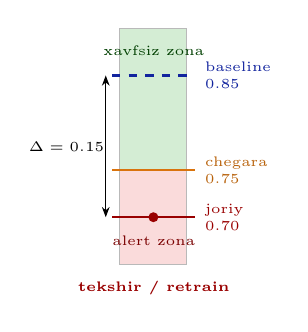
\begin{tikzpicture}[font=\tiny]
        \fill[cokfill]    (0,1.20) rectangle (0.85,3.00);
        \fill[calertfill] (0,0.00) rectangle (0.85,1.20);
        \draw[gray!55] (0,0) rectangle (0.85,3.0);

        \draw[cnublue, dashed, thick]
          (-0.10,2.40)--(0.95,2.40)
          node[right, cnublue, align=left]{baseline\\$0.85$};

        \draw[cwarn, thick]
          (-0.10,1.20)--(0.95,1.20)
          node[right, cwarn!85!black, align=left]{chegara\\$0.75$};

        \fill[deepred] (0.425,0.60) circle (1.8pt);
        \draw[deepred, thick]
          (-0.10,0.60)--(0.95,0.60)
          node[right, deepred, align=left]{joriy\\$0.70$};

        \draw[{Stealth[length=1.3mm]}-{Stealth[length=1.3mm]}, black]
          (-0.18,2.40)--(-0.18,0.60)
          node[midway, left, fill=white, inner sep=0.4pt]{$\Delta=0.15$};

        \node[deepgreen!55!black, font=\tiny] at (0.43,2.72){xavfsiz zona};
        \node[deepred!80!black, font=\tiny] at (0.43,0.30){alert zona};
        \node[deepred, font=\tiny\bfseries] at (0.43,-0.30){tekshir / retrain};
      \end{tikzpicture}
    \end{column}
  \end{columns}
\end{frame}

% ----------------------------------------------------------------
% [J3] SIZNING VAZIFANGIZ
% ----------------------------------------------------------------
\begin{frame}{Sizning vazifangiz: ogohlantirish kerakmi?}
  \small

  \begin{tcolorbox}[warnbox,title=Savol,top=2pt,bottom=2pt]
    Baseline $F_{1,\text{base}} = 0.88$;
    joriy $F_{1,\text{joriy}} = 0.82$;
    chegara $\tau = 0.10$.\\[3pt]
    \textbf{$\Delta = ?$ \qquad Ogohlantirish ishga tushadimi?}
  \end{tcolorbox}

  \pause
  \vspace{-5pt}

  \begin{columns}[T,totalwidth=\textwidth]
    \begin{column}{0.58\textwidth}
      \begin{tcolorbox}[okbox,title=Javob,top=2pt,bottom=2pt]
        \small
        \[
          \Delta
          =
          F_{1,\text{base}} - F_{1,\text{joriy}}
          =
          0.88 - 0.82
          =
          0.06
        \]

        \[
          0.06 < 0.10 = \tau
          \quad\Rightarrow\quad
          \textbf{ogohlantirish yo\uzq{}q}
        \]

        \footnotesize
        Pasayish bor, lekin chegara buzilmadi. Demak, holatni kuzatishda
        davom etamiz. $\tau$ juda past qo\uzq{}yilsa, behuda ogohlantirishlar
        ko\uzq{}payadi; juda yuqori qo\uzq{}yilsa, muammo kech aniqlanadi.
      \end{tcolorbox}
    \end{column}

    \begin{column}{0.40\textwidth}
      \centering
      {\footnotesize\textbf{Chegara bilan solishtirish}}\\[2pt]

      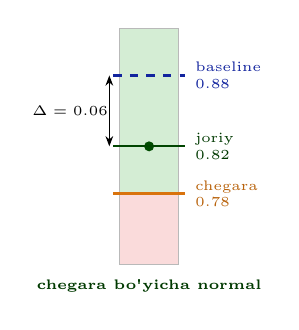
\begin{tikzpicture}[font=\tiny]
        \fill[cokfill]    (0,0.9) rectangle (0.75,3.0);
        \fill[calertfill] (0,0)   rectangle (0.75,0.9);
        \draw[gray!55] (0,0) rectangle (0.75,3.0);

        \draw[cnublue, dashed, thick]
          (-0.08,2.4)--(0.83,2.4)
          node[right, cnublue, align=left]{baseline\\$0.88$};

        \draw[cwarn, thick]
          (-0.08,0.9)--(0.83,0.9)
          node[right, cwarn!85!black, align=left]{chegara\\$0.78$};

        \fill[deepgreen!65!black] (0.375,1.5) circle (1.8pt);
        \draw[deepgreen!60!black, thick]
          (-0.08,1.5)--(0.83,1.5)
          node[right, deepgreen!50!black, align=left]{joriy\\$0.82$};

        \draw[{Stealth[length=1.3mm]}-{Stealth[length=1.3mm]}, black]
          (-0.13,2.4)--(-0.13,1.5)
          node[midway, left, fill=white, inner sep=0.4pt]{$\Delta=0.06$};

        \node[deepgreen!50!black, font=\tiny\bfseries]
          at (0.375,-0.28){chegara bo\uzq{}yicha normal};
      \end{tikzpicture}
    \end{column}
  \end{columns}
\end{frame}

% ----------------------------------------------------------------
% [K3] KOD <-> FORMULA  [fragile]
% ----------------------------------------------------------------
\begin{frame}[fragile]{Kod $\leftrightarrow$ formula: sifat pasayishini tekshirish}
  \small

  \begin{columns}[T,totalwidth=\textwidth]
    \begin{column}{0.59\textwidth}
\begin{lstlisting}[basicstyle=\ttfamily\scriptsize]
BASELINE_F1 = 0.85
TAU = 0.10

def check_quality_drop(current_f1):
    delta = BASELINE_F1 - current_f1

    if delta >= TAU:
        return "alert"    # sababni tekshir

    return "ok"

print(check_quality_drop(0.70))  # alert
\end{lstlisting}
    \end{column}

    \begin{column}{0.38\textwidth}
      \textbf{Kod $\to$ formula}\\[3pt]

      \footnotesize
      \renewcommand{\arraystretch}{1.12}
      \begin{tabular}{p{2.35cm}p{1.95cm}}
        \toprule
        \textbf{Kod} & \textbf{Formula} \\
        \midrule
        \texttt{delta} & $\Delta$ \\
        \texttt{BASELINE\_F1} & $F_{1,\text{base}}$ \\
        \texttt{current\_f1} & $F_{1,\text{joriy}}$ \\
        \texttt{delta >= TAU} & $\Delta \ge \tau$ \\
        \bottomrule
      \end{tabular}

      \vspace{5pt}

      \begin{tcolorbox}[okbox,top=2pt,bottom=2pt,left=3pt,right=3pt]
        \footnotesize
        Davriy ish bu funksiyani yangi yorliqlangan namunada ishga tushiradi.
        \texttt{alert} chiqsa, avval sabab tekshiriladi; kerak bo\uzq{}lsa
        retrain yoki rollback qilinadi.
      \end{tcolorbox}
    \end{column}
  \end{columns}
\end{frame}

% ----------------------------------------------------------------
% [L3] TUZOG\uzq{}
% ----------------------------------------------------------------
\begin{frame}{Versiyalash tuzog\uzq{}i: eski model saqlanmagan}
  \small

  \begin{columns}[T,totalwidth=\textwidth]
    \begin{column}{0.51\textwidth}
      \begin{tcolorbox}[warnbox,title={Muammo},top=2pt,bottom=2pt]
        \footnotesize
        Yangi model production muhitida yomon ishlasa, lekin eski barqaror
        versiya saqlanmagan bo\uzq{}lsa, tezda ortga qaytish
        (\textit{rollback}) qiyin bo\uzq{}ladi.\\[3pt]

        Natijada xizmat sifati pasaygan holatda qolishi mumkin.
      \end{tcolorbox}

      \vspace{4pt}

      \begin{tcolorbox}[defbox,top=2pt,bottom=2pt]
        \footnotesize
        \textbf{Tuzoq:}
        faqat \texttt{model.pt} yoki \texttt{model.pkl} faylini almashtirish
        yetarli emas; u qaysi kod, qaysi tokenizer va qaysi data bilan
        olingani ham muhim.
      \end{tcolorbox}
    \end{column}

    \begin{column}{0.46\textwidth}
      \begin{tcolorbox}[okbox,title={Yechim: model reyestri},top=2pt,bottom=2pt]
        \footnotesize
        Har bir versiya uchun quyidagilar saqlanadi:
        \begin{itemize}\setlength\itemsep{1pt}
          \item model artefakti: \texttt{v1}, \texttt{v2}, \dots;
          \item tokenizer/preprocessing va config;
          \item metrikalar, sana, kod/data versiyasi;
          \item holat: \textit{staging}, \textit{production}, \textit{archived}.
        \end{itemize}
      \end{tcolorbox}

      \vspace{4pt}

      \begin{tcolorbox}[okbox,top=2pt,bottom=2pt]
        \footnotesize
        \textbf{Rollback g\uzq{}oyasi:}
        \texttt{v2} yomon ishlasa, xizmat tezda eski barqaror
        \texttt{v1} versiyasiga qaytariladi.
      \end{tcolorbox}
    \end{column}
  \end{columns}
\end{frame}

% ================================================================
\section[CI/CD]{CI/CD pipeline}
% ================================================================

% ----------------------------------------------------------------
% [F4] INTUITSIYA
% ----------------------------------------------------------------
\begin{frame}{Intuitsiya: qo\uzq{}lda emas, avtomatik pipeline}
  \small

  \begin{columns}[T,totalwidth=\textwidth]
    \begin{column}{0.52\textwidth}
      Har bir o\uzq{}zgarishdan keyin testlarni qo\uzq{}lda ishga tushirish,
      Docker image qurish va xizmatni yangilash sekin hamda xatoga moyil.\\[5pt]

      \textbf{CI/CD pipeline} --- kod o\uzq{}zgarganda tekshirish, qurish va
      joylashtirish bosqichlarini avtomatik bajaradigan jarayon.\\[6pt]

      \textbf{CI} (\textit{Continuous Integration}) ---
      kodni tekshirish: testlar va build.\\[3pt]

      \textbf{CD} (\textit{Continuous Delivery/Deployment}) ---
      tayyor versiyani yetkazish yoki muhitga joylashtirish.
    \end{column}

    \begin{column}{0.45\textwidth}
      \begin{tcolorbox}[defbox,top=2pt,bottom=2pt,left=4pt,right=4pt]
        \centering
        \footnotesize
        \textbf{Pipeline oqimi}\\[4pt]
        kod o\uzq{}zgaradi\\[-1pt]
        $\Downarrow$\\[-1pt]
        testlar ishlaydi\\[-1pt]
        $\Downarrow$\\[-1pt]
        Docker image quriladi\\[-1pt]
        $\Downarrow$\\[-1pt]
        xizmat yangilanadi
      \end{tcolorbox}

      \vspace{4pt}

      \begin{tcolorbox}[okbox,top=2pt,bottom=2pt,left=4pt,right=4pt]
        \footnotesize
        Biz amaliyotlarda yozgan \texttt{assert}lar --- CI testlarining
        sodda ko\uzq{}rinishi. Pipeline ularni avtomatik tekshiradi.
      \end{tcolorbox}
    \end{column}
  \end{columns}
\end{frame}
% ----------------------------------------------------------------
% [G4] RASMIY TA\uzq{}RIF + BUNDA
% ----------------------------------------------------------------
\begin{frame}{CI/CD: rasmiy ta\uzq{}rif}
  \small

  \begin{tcolorbox}[defbox,top=2pt,bottom=2pt,left=4pt,right=4pt]
    \footnotesize
    \textbf{CI/CD} --- koddagi o\uzq{}zgarishlarni avtomatik tekshirish,
    qurish va muhitga joylashtirishni boshqaradigan jarayon.
  \end{tcolorbox}

  \vspace{3pt}

  \begin{center}
  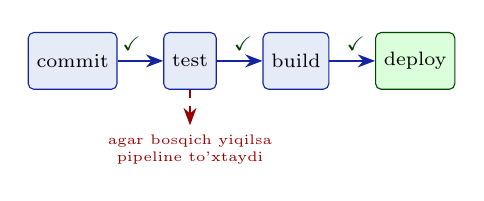
\begin{tikzpicture}[node distance=0.58cm]
    \node[flowbox] (c) {commit};
    \node[flowbox, right=of c] (t) {test};
    \node[flowbox, right=of t] (b) {build};
    \node[flowbox, fill=green!14, draw=deepgreen!60!black, right=of b] (d) {deploy};

    \draw[flowarr] (c)--(t);
    \draw[flowarr] (t)--(b);
    \draw[flowarr] (b)--(d);

    \node[deepgreen!55!black, font=\scriptsize] at ($(c)!0.5!(t)+(0,0.22)$) {$\checkmark$};
    \node[deepgreen!55!black, font=\scriptsize] at ($(t)!0.5!(b)+(0,0.22)$) {$\checkmark$};
    \node[deepgreen!55!black, font=\scriptsize] at ($(b)!0.5!(d)+(0,0.22)$) {$\checkmark$};

    \node[deepred, font=\tiny, below=0.45cm of t, align=center] (st)
      {agar bosqich yiqilsa\\ pipeline to'xtaydi};
    \draw[backarr] (t.south)--(st.north);
  \end{tikzpicture}
  \end{center}

  \vspace{2pt}

  \begin{tcolorbox}[okbox,top=2pt,bottom=2pt,left=4pt,right=4pt]
    \scriptsize
    \textbf{Bosqichlar:}
    \textit{commit} --- kodni repozitoriyga yuborish;
    \textit{test} --- avtomatik tekshiruvlar (\texttt{assert}, unit test);
    \textit{build} --- artefakt yoki Docker image qurish;
    \textit{deploy} --- tayyor versiyani staging yoki production muhitiga joylashtirish.
  \end{tcolorbox}
\end{frame}

% ----------------------------------------------------------------
% [H4] KELTIRIB CHIQARISH
% ----------------------------------------------------------------
\begin{frame}{Asoslash: nega avtomatlashtirish kerak?}
  \small

  \begin{columns}[T,totalwidth=\textwidth]
    \begin{column}{0.48\textwidth}
      \begin{tcolorbox}[warnbox,title={Qo\uzq{}lda bajarilsa},top=2pt,bottom=2pt]
        \footnotesize
        Har o\uzq{}zgarishdan keyin test, build va deploy bosqichlarini
        qo\uzq{}lda bajarish:
        \begin{itemize}\setlength\itemsep{2pt}
          \item sekin va takroriy ish;
          \item inson xatosiga moyil;
          \item xatoli kodni kech aniqlaydi.
        \end{itemize}
      \end{tcolorbox}
    \end{column}

    \begin{column}{0.49\textwidth}
      \begin{tcolorbox}[okbox,title={CI/CD pipeline bo\uzq{}lsa},top=2pt,bottom=2pt]
        \footnotesize
        Har bir commitdan keyin jarayon avtomatik ishlaydi:
        \begin{enumerate}\setlength\itemsep{2pt}
          \item testlar ishga tushadi;
          \item testlar o\uzq{}tsa, Docker image quriladi;
          \item build muvaffaqiyatli bo\uzq{}lsa, deploy bajariladi;
          \item bosqich yiqilsa, pipeline to\uzq{}xtaydi.
        \end{enumerate}
      \end{tcolorbox}
    \end{column}
  \end{columns}

  \vspace{4pt}

  \begin{tcolorbox}[defbox,top=2pt,bottom=2pt,left=4pt,right=4pt]
    \footnotesize
    \textbf{Xulosa:}
    CI/CD sifat nazorat bosqichlarini avtomatlashtiradi.
    Kursdagi \texttt{assert}lar esa shu avtomatik testlarning sodda ko\uzq{}rinishi:
    kod o\uzq{}zgarsa, ular xatoni erta ushlashga yordam beradi.
  \end{tcolorbox}
\end{frame}

% ----------------------------------------------------------------
% [I4] QO\uzq{}LDA MISOL (ILLYUSTRATIV)
% ----------------------------------------------------------------
\begin{frame}{Qo\uzq{}lda misol: pipeline bosqichlari}
  \small

  \begin{tcolorbox}[defbox,top=2pt,bottom=2pt,left=4pt,right=4pt]
    \footnotesize
    \textbf{Faraz:} pipeline ketma-ket ishlaydi.
    Test $30$ s, build $90$ s, deploy $20$ s.
  \end{tcolorbox}

  \vspace{3pt}

  \begin{center}
  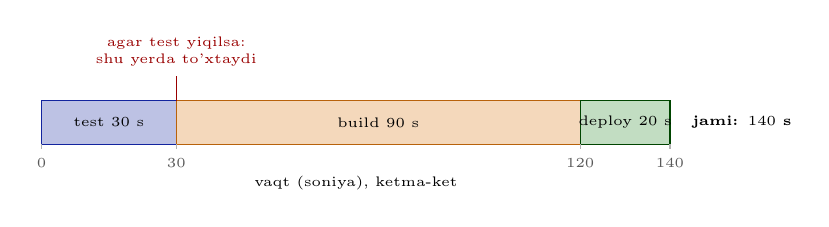
\begin{tikzpicture}[font=\tiny]
    \def\s{0.057}
    \def\h{0.55}

    % bar segments
    \fill[cnublue!28, draw=cnublue] (0,0) rectangle ({30*\s},\h);
    \node at ({15*\s},{\h/2}) {test $30$ s};

    \fill[cwarn!28, draw=cwarn!85!black] ({30*\s},0) rectangle ({120*\s},\h);
    \node at ({75*\s},{\h/2}) {build $90$ s};

    \fill[deepgreen!24, draw=deepgreen!60!black] ({120*\s},0) rectangle ({140*\s},\h);
    \node at ({130*\s},{\h/2}) {deploy $20$ s};

    % ticks
    \foreach \tt in {0,30,120,140}{
      \draw[gray!60] ({\tt*\s},-0.06) -- ({\tt*\s},0);
      \node[below=0pt, gray!70!black] at ({\tt*\s},-0.06) {\tt};
    }

    % total label
    \node[right] at ({140*\s+0.16},{\h/2}) {\textbf{jami: $140$ s}};

    % axis label
    \node[below=0.28cm] at ({70*\s},0) {vaqt (soniya), ketma-ket};

    % fail marker
    \draw[deepred, thin] ({30*\s},\h) -- ++(0,0.32);
    \node[above, deepred, align=center] at ({30*\s},{\h+0.32})
      {agar test yiqilsa:\\ shu yerda to'xtaydi};
  \end{tikzpicture}
  \end{center}

  \vspace{3pt}

  \begin{columns}[T,totalwidth=\textwidth]
    \begin{column}{0.55\textwidth}
      \footnotesize
      \textbf{To\uzq{}liq muvaffaqiyatli pipeline:} $30 + 90 + 20 = 140$ s.\\[3pt]
      \textbf{Agar test yiqilsa:} pipeline taxminan $30$ s da to\uzq{}xtaydi,
      build va deploy bajarilmaydi. Shuning uchun \textbf{xatoli kod}
      ishlab chiqarish muhitiga chiqmaydi.
    \end{column}

    \begin{column}{0.41\textwidth}
      \begin{tcolorbox}[okbox,top=2pt,bottom=2pt,left=4pt,right=4pt]
        \footnotesize
        \textbf{Asosiy foyda:}
        dasturchi xato haqida tezkor qayta aloqa oladi.
        Muammo bir necha daqiqada bilinadi, kunlab kechikmaydi.
      \end{tcolorbox}
    \end{column}
  \end{columns}

  \vspace{2pt}
  {\scriptsize
  \textbf{Eslatma:} bu soddalashtirilgan ketma-ket misol.
  Amalda ayrim testlar parallel ishlashi mumkin.
  }
\end{frame}

% ----------------------------------------------------------------
% [J4] SIZNING VAZIFANGIZ
% ----------------------------------------------------------------
\begin{frame}{Sizning vazifangiz: testdan o\uzq{}tmadi}
  \small

  \begin{tcolorbox}[warnbox,title=Savol,top=2pt,bottom=2pt]
    Pipeline jarayonida test bosqichi muvaffaqiyatsiz tugadi:
    bitta \texttt{assert} o\uzq{}tmadi.\\[3pt]
    \textbf{Keyingi bosqichlar --- build va deploy --- bajariladimi?}
  \end{tcolorbox}

  \pause

  \vspace{3pt}

  \begin{tcolorbox}[okbox,title=Javob,top=2pt,bottom=2pt]
    \small
    \textbf{Yo\uzq{}q.} Pipeline test bosqichida to\uzq{}xtaydi;
    \textbf{build} va \textbf{deploy} bajarilmaydi.\\[4pt]

    \footnotesize
    Sababi: testdan o\uzq{}tmagan koddan Docker image qurilsa va u production
    muhitiga chiqarilsa, xatoli versiya foydalanuvchiga yetib borishi mumkin.\\[3pt]

    \textbf{Keyingi qadam:} xatoni tuzatish $\rightarrow$ qayta commit qilish
    $\rightarrow$ pipeline testlarni yana ishga tushiradi.
  \end{tcolorbox}

  \vspace{3pt}

  {\scriptsize
  \textbf{Xulosa:} \texttt{assert} va unit testlar CI/CD pipeline dagi birinchi
  sifat nazorati hisoblanadi.
  }
\end{frame}

% ----------------------------------------------------------------
% [K4] KOD <-> FORMULA  [fragile]
% ----------------------------------------------------------------
\begin{frame}[fragile]{Kod $\leftrightarrow$ bosqich: CI/CD pipeline (YAML)}
  \small

  \begin{columns}[T,totalwidth=\textwidth]
    \begin{column}{0.60\textwidth}
\begin{lstlisting}[basicstyle=\ttfamily\scriptsize]
# .github/workflows/ci.yml
on:
  push:
    branches: [main]

jobs:
  pipeline:
    runs-on: ubuntu-latest
    steps:
      - uses: actions/checkout@v4
      - run: pytest
      - run: docker build -t nlp-api:latest .
      - run: ./deploy.sh
\end{lstlisting}
    \end{column}

    \begin{column}{0.37\textwidth}
      \textbf{Qator $\to$ bosqich}\\[3pt]

      \footnotesize
      \renewcommand{\arraystretch}{1.12}
      \begin{tabular}{p{2.05cm}p{1.65cm}}
        \toprule
        \textbf{Qator} & \textbf{Bosqich} \\
        \midrule
        \texttt{checkout} & kodni olish \\
        \texttt{pytest} & test \\
        \texttt{docker build} & build \\
        \texttt{deploy.sh} & deploy \\
        \bottomrule
      \end{tabular}

      \vspace{5pt}

      \begin{tcolorbox}[okbox,top=2pt,bottom=2pt,left=3pt,right=3pt]
        \footnotesize
        \texttt{main} branchga \texttt{push} qilinganda pipeline avtomatik ishga tushadi.
        Biror bosqich muvaffaqiyatsiz bo\uzq{}lsa, keyingi bosqichlar bajarilmaydi.
      \end{tcolorbox}

      \vspace{3pt}
      {\scriptsize
      \textbf{Eslatma:} production deploy odatda maxfiy kalitlar va ruxsat
      nazorati bilan bajariladi.
      }
    \end{column}
  \end{columns}
\end{frame}

% ----------------------------------------------------------------
% [L4] TUZOG\uzq{}
% ----------------------------------------------------------------
\begin{frame}{CI/CD tuzog\uzq{}i: testlarsiz pipeline}
  \small

  \begin{columns}[T,totalwidth=\textwidth]
    \begin{column}{0.51\textwidth}
      \begin{tcolorbox}[warnbox,title={Muammo: faqat deploy avtomatik},top=2pt,bottom=2pt]
        \footnotesize
        Agar pipeline faqat deploy qilsa, lekin testlardan o\uzq{}tkazmasa,
        xatoli kod ishlab chiqarish muhitiga tezroq chiqib ketadi.\\[3pt]

        Demak, avtomatlashtirishning o\uzq{}zi yetarli emas:
        u \textbf{sifat nazorati} bilan birga bo\uzq{}lishi kerak.
      \end{tcolorbox}

      \vspace{4pt}

      \begin{tcolorbox}[defbox,top=2pt,bottom=2pt,left=4pt,right=4pt]
        \footnotesize
        \textbf{Noto\uzq{}g\uzq{}ri oqim:}\\[2pt]
        \centering
        commit $\rightarrow$ build $\rightarrow$ deploy
      \end{tcolorbox}
    \end{column}

    \begin{column}{0.46\textwidth}
      \begin{tcolorbox}[okbox,title={Yechim},top=2pt,bottom=2pt]
        \footnotesize
        Deploydan oldin majburiy test bosqichi qo\uzq{}yiladi:
        \[
          \text{commit}
          \rightarrow
          \text{test}
          \rightarrow
          \text{build}
          \rightarrow
          \text{deploy}
        \]
        Test muvaffaqiyatsiz bo\uzq{}lsa, pipeline to\uzq{}xtaydi.
      \end{tcolorbox}

      \vspace{4pt}

      \begin{tcolorbox}[okbox,top=2pt,bottom=2pt,left=4pt,right=4pt]
        \footnotesize
        \textbf{Deploydan keyin:}
        nazorat sinovi (\textit{smoke test}) bajariladi:
        API ishga tushdimi, \texttt{/health} javob berdimi,
        \texttt{/predict} oddiy so\uzq{}rovga javob qaytardimi?
      \end{tcolorbox}
    \end{column}
  \end{columns}
\end{frame}

% ================================================================
\section[Xulosa]{Xulosa, capstone himoyasi va keyingi yo\uzq{}l}
% ================================================================

% ----------------------------------------------------------------
% [M] O\uzq{}ZBEK TILIGA XOSLIK (majburiy arxetip)
% ----------------------------------------------------------------
\begin{frame}{O\uzq{}zbek tili uchun NLP: ekotizim va ochiq muammolar}
  \small
\vspace{-2mm}
  \begin{columns}[T,totalwidth=\textwidth]
    \begin{column}{0.50\textwidth}
      \textbf{1. Mavjud yo\uzq{}nalishlar}\\[3pt]

      O\uzq{}zbek tili uchun ochiq modellar va baholash resurslari paydo
      bo\uzq{}lmoqda: UzBERT, BERTbek, UzLiB kabi tashabbuslar.\\[4pt]

      Lekin ingliz tiliga nisbatan resurslar, benchmarklar va domenga xos
      tayyor yechimlar hali cheklangan.

      \vspace{-4pt}

      \begin{tcolorbox}[warnbox,title={Ochiq muammolar},top=2pt,bottom=2pt,boxsep=0.1mm]
        \footnotesize
        \begin{itemize}\setlength\itemsep{2pt}
          \item sifatli yorliqlangan ma\uzq{}lumotlar kamligi;
          \item morfologiya va imlo uchun ishonchli vositalar;
          \item huquq, tibbiyot, ta\uzq{}lim kabi domenlarga xos modellar;
          \item standart baholash to\uzq{}plamlari va benchmarklar.
        \end{itemize}
      \end{tcolorbox}
    \end{column}

    \begin{column}{0.46\textwidth}
      \textbf{2. Sizning keyingi hissangiz}\\[3pt]

      Kursda qurgan modullaringiz --- amaliy loyiha va ilmiy izlanishlar
      uchun boshlang\uzq{}ich poydevor.

      \vspace{-4pt}

      \begin{tcolorbox}[okbox,title={Amaliy yo\uzq{}nalishlar},top=2pt,bottom=2pt,boxsep=0.1mm]
        \footnotesize
        \begin{enumerate}\setlength\itemsep{2pt}
          \item kichik, lekin toza o\uzq{}zbek korpus yoki benchmark yaratish;
          \item ochiq modelni aniq vazifaga moslab fine-tune qilish;
          \item RAG yoki agent asosida domenga xos yordamchi qurish;
          \item model, kod va baholash natijalarini hujjatlashtirib ulashish.
        \end{enumerate}
      \end{tcolorbox}

      \vspace{-4pt}

      \begin{tcolorbox}[defbox,top=2pt,bottom=2pt,boxsep=0.1mm]
        \footnotesize
        \textbf{Kalit fikr:}
        kichik, sifatli va qayta ishlatiladigan resurs katta modeldan ham
        foydaliroq bo\uzq{}lishi mumkin.
      \end{tcolorbox}
    \end{column}
  \end{columns}
\end{frame}

% ----------------------------------------------------------------
% [N] SINTEZ
% ----------------------------------------------------------------
\begin{frame}{Sintez: notebookdan ishlab chiqarish xizmatigacha}
  \small

  \begin{center}
  \renewcommand{\arraystretch}{1.16}
  \begin{tabular}{p{2cm}p{4.45cm}p{5.95cm}}
    \toprule
    \textbf{Jihat} & \textbf{Notebook / prototip} & \textbf{Ishlab chiqarish / MLOps} \\
    \midrule
    Maqsad &
    sinash, o\uzq{}rganish, tajriba qilish &
    foydalanuvchiga ishonchli xizmat berish \\

    Muhit &
    shaxsiy kompyuter yoki Kaggle &
    Docker orqali barqarorlashtirilgan muhit \\

    Ishlash tartibi &
    qo\uzq{}lda ishga tushirish &
    API orqali doimiy xizmat ko\uzq{}rsatish \\

    Sifat nazorati &
    bir martalik baholash &
    monitoring, alert va drift indikatorlari \\

    Yangilash &
    qo\uzq{}lda o\uzq{}zgartirish &
    CI/CD, model reyestri va rollback \\
    \bottomrule
  \end{tabular}
  \end{center}

  \vspace{5pt}

  \begin{tcolorbox}[okbox,top=2pt,bottom=2pt,left=4pt,right=4pt]
    \footnotesize
    \textbf{Asosiy g\uzq{}oya:}
    MLOps notebookdagi modelni \textbf{ishonchli}, \textbf{takror ishlab bo\uzq{}ladigan}
    va \textbf{yangilanadigan} xizmatga aylantiradi:
    \textit{train} $\to$ \textit{package} $\to$ \textit{serve} $\to$ \textit{monitor},
    Docker, model reyestri va CI/CD.
  \end{tcolorbox}
\end{frame}

% ----------------------------------------------------------------
% [O] SEMINAL MANBA + MUHOKAMA SAVOLI
% ----------------------------------------------------------------
\begin{frame}{Tayanch manba: Sculley va boshqalar (2015)}
  \small

  \begin{tcolorbox}[defbox,top=2pt,bottom=2pt,left=4pt,right=4pt]
    \footnotesize
    \textbf{Manba:}
    Sculley, D., va boshq.\ (2015).
    \textbf{Hidden Technical Debt in Machine Learning Systems.}
    \textit{NeurIPS 28.}
  \end{tcolorbox}

  \vspace{4pt}

  \textbf{Nega bu maqola muhim?}
  \begin{itemize}\setlength\itemsep{3pt}
    \item ML tizimida model kodi faqat kichik qism; ma\uzq{}lumot, serving,
          monitoring, konfiguratsiya va test infratuzilmasi ham muhim.
    \item ``Yashirin texnik qarz'' --- tizim hozir ishlayotgandek ko\uzq{}rinsa ham,
          keyin uni saqlash, yangilash va tekshirish qimmatlashib borishi.
    \item Deploy, monitoring, versiyalash va CI/CD --- shu qarzni kamaytirishga
          yordam beradigan MLOps amaliyotlari.
  \end{itemize}

  \vspace{4pt}

  \begin{tcolorbox}[warnbox,title={Muhokama savoli},top=2pt,bottom=2pt,left=4pt,right=4pt]
    \footnotesize
    O\uzq{}zbek tilidagi NLP xizmati uchun qaysi ``yashirin texnik qarz''
    xavfliroq bo\uzq{}lishi mumkin:
    \textbf{data drift}, \textbf{yorliqlangan ma\uzq{}lumot kamligi} yoki
    \textbf{tokenizer/preprocessing mos kelmasligi}? Nega?
  \end{tcolorbox}
\end{frame}

% ----------------------------------------------------------------
% [P] MAQSADLAR BAJARILDI
% ----------------------------------------------------------------
\begin{frame}{Bugungi maqsadlar bajarildi}
  \small

  \begin{enumerate}\setlength\itemsep{7pt}
    \item \bajarildi
    Modelni ishlab chiqarish muhitiga joriy etish bosqichlarini
    \textbf{tushuntira olasiz}:\\
    \textit{train} $\to$ \textit{package} $\to$ \textit{serve} $\to$ \textit{monitor}.

    \item \bajarildi
    FastAPI va Docker yordamida modelni API ko\uzq{}rinishidagi xizmatga
    aylantirish g\uzq{}oyasini \textbf{tushuntira olasiz}.

    \item \bajarildi
    Monitoring, sifat pasayishi, siljish (\textit{drift}) va model
    versiyalash nima uchun kerakligini \textbf{tushuntira olasiz}.

    \item \bajarildi
    CI/CD pipeline NLP loyihasini avtomatlashtirishda qanday ishlashini
    va o\uzq{}zbek NLP ekotizimida keyingi yo\uzq{}nalishlarni
    \textbf{tushuntira olasiz}.
  \end{enumerate}

  \vspace{5pt}

  \begin{tcolorbox}[okbox,top=2pt,bottom=2pt,left=4pt,right=4pt]
    \footnotesize
    \textbf{Yakuniy fikr:}
    notebookdagi model faqat prototip; MLOps uni ishonchli, kuzatiladigan
    va yangilanadigan xizmatga aylantiradi.
  \end{tcolorbox}
\end{frame}

% ----------------------------------------------------------------
% [Q] KO\uzq{}PRIK: CAPSTONE HIMOYASI (keyingi P ga emas --- kurs yakuni)
% ----------------------------------------------------------------
\begin{frame}{Yakuniy loyiha himoyasi: ``O\uzq{}zbek hujjat yordamchisi''}
  \small

  \begin{center}
  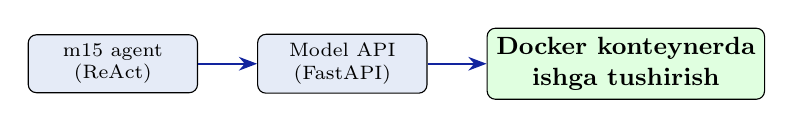
\begin{tikzpicture}[
      mod/.style={draw, fill=cnubluebg, rounded corners=3pt,
                  minimum width=2.15cm, minimum height=0.72cm,
                  font=\scriptsize, align=center},
      fin/.style={draw, fill=green!12, rounded corners=3pt,
                  minimum width=2.55cm, minimum height=0.72cm,
                  font=\small\bfseries, align=center},
      arr/.style={-{Stealth}, thick, color=cnublue}
  ]
    \node[mod] (m15) {m15 agent\\(ReAct)};
    \node[mod, right=0.75cm of m15] (api) {Model API\\(FastAPI)};
    \node[fin, right=0.75cm of api] (dep) {Docker konteynerda\\ishga tushirish};
    \draw[arr] (m15)--(api);
    \draw[arr] (api)--(dep);
  \end{tikzpicture}
  \end{center}

  \vspace{4pt}

  \begin{columns}[T,totalwidth=\textwidth]
    \begin{column}{0.54\textwidth}
      \textbf{Himoyada ko\uzq{}rsating:}\\[3pt]
      \begin{itemize}\setlength\itemsep{3pt}
        \item \texttt{DocumentAssistantAgent} ning jonli ishlashi
              (o\uzq{}zbekcha so\uzq{}rov bilan).
        \item API orqali modelga murojaat:
              masalan \texttt{POST /predict} yoki loyiha endpointi.
        \item Tizimni Docker orqali ishga tushirish va xizmatning
              barqaror ishlashini qisqa ko\uzq{}rsatish.
      \end{itemize}
    \end{column}

    \begin{column}{0.42\textwidth}
      \begin{tcolorbox}[okbox,title={Tayyorlab keling},top=2pt,bottom=2pt,left=4pt,right=4pt]
        \footnotesize
        Bitta ishlaydigan tizimni yaxlit tarzda tushuntiring:
        \textbf{modullar} (m01--m15),
        \textbf{API},
        \textbf{Docker} va
        \textbf{MLOps} g\uzq{}oyalari qanday bog\uzq{}langanini ko\uzq{}rsating.
      \end{tcolorbox}

      \vspace{4pt}

      \begin{tcolorbox}[defbox,top=2pt,bottom=2pt,left=4pt,right=4pt]
        \footnotesize
        \textbf{Asosiy mezon:}
        alohida qismlar emas, balki
        \textbf{oxirigacha ishlaydigan quvur}
        (\textit{agent} $\rightarrow$ \textit{API} $\rightarrow$ \textit{Docker})
        ko\uzq{}rsatilishi muhim.
      \end{tcolorbox}
    \end{column}
  \end{columns}
\end{frame}

% ----------------------------------------------------------------
% [Q2] KURS YO'LI (butun NLP oqimi --- qo'shilgan, kurs finali)
% ----------------------------------------------------------------
\begin{frame}{Kurs yo\uzq{}li: matnni tozalashdan ishonchli xizmatgacha}
  \begin{center}
  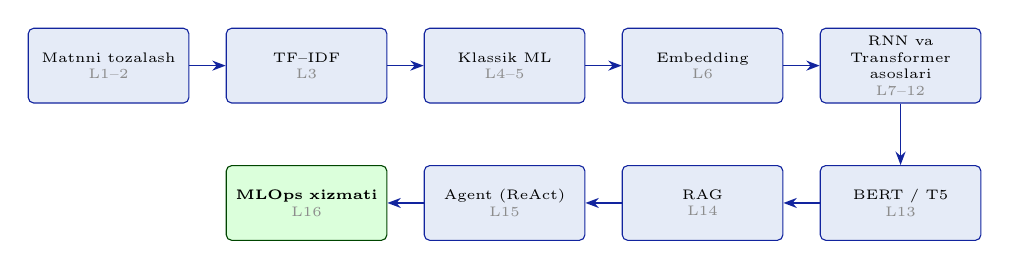
\begin{tikzpicture}[
      arcbox/.style={draw=cnublue, fill=cnubluebg, rounded corners=2pt,
                 minimum height=0.95cm, text width=1.9cm, align=center,
                 font=\tiny, inner sep=2pt},
      arcfin/.style={arcbox, fill=green!14, draw=deepgreen!60!black},
      a/.style={-{Stealth[length=1.7mm]}, semithick, cnublue}
    ]
    % 1-qator
    \node[arcbox] (n1) {Matnni tozalash\\ \textcolor{halfgray}{L1--2}};
    \node[arcbox, right=0.46cm of n1] (n2) {TF--IDF\\ \textcolor{halfgray}{L3}};
    \node[arcbox, right=0.46cm of n2] (n3) {Klassik ML\\ \textcolor{halfgray}{L4--5}};
    \node[arcbox, right=0.46cm of n3] (n4) {Embedding\\ \textcolor{halfgray}{L6}};
    \node[arcbox, right=0.46cm of n4] (n5) {RNN va\\ Transformer asoslari\\ \textcolor{halfgray}{L7--12}};
    \draw[a] (n1)--(n2);
    \draw[a] (n2)--(n3);
    \draw[a] (n3)--(n4);
    \draw[a] (n4)--(n5);

    % pastga
    \node[arcbox, below=0.78cm of n5] (n6) {BERT / T5\\ \textcolor{halfgray}{L13}};
    \draw[a] (n5)--(n6);

    % 2-qator
    \node[arcbox, left=0.46cm of n6] (n7) {RAG\\ \textcolor{halfgray}{L14}};
    \node[arcbox, left=0.46cm of n7] (n8) {Agent (ReAct)\\ \textcolor{halfgray}{L15}};
    \node[arcfin, left=0.46cm of n8] (n9) {\textbf{MLOps xizmati}\\ \textcolor{halfgray}{L16}};
    \draw[a] (n6)--(n7);
    \draw[a] (n7)--(n8);
    \draw[a] (n8)--(n9);
  \end{tikzpicture}
  \end{center}

  \vspace{3pt}

  \begin{tcolorbox}[okbox,title={Bitta zanjir --- kurs yakuni},top=2pt,bottom=2pt]
    \footnotesize
    Har bir ma\uzq{}ruza umumiy yo\uzq{}lning bir qismi edi:
    \textbf{matnni tayyorlash} (L1--6),
    \textbf{modellarni tushunish va o\uzq{}qitish} (L7--13),
    \textbf{bilimga tayangan tizimlar} (L14--15)
    va nihoyat \textbf{ishonchli xizmat} (L16).
    Endi sizda to\uzq{}liq NLP tizimini qurish uchun yaxlit tasavvur bor.
  \end{tcolorbox}
\end{frame}

% ----------------------------------------------------------------
% [R] ADABIYOTLAR + KURS YAKUNI
% ----------------------------------------------------------------
\begin{frame}{Adabiyotlar va kurs yakuni}
  \small

  \begin{enumerate}\setlength\itemsep{4pt}
    \item Sculley, D., va boshq.\ (2015).
          \textit{Hidden Technical Debt in Machine Learning Systems}.
          NeurIPS 28.

    \item Huyen, C.\ (2022).
          \textit{Designing Machine Learning Systems}.
          O'Reilly.

    \item FastAPI rasmiy hujjatlari va Docker Docs ---
          API yaratish hamda Docker bilan konteynerlashtirish.

    \item Google Cloud va Microsoft Azure MLOps qo\uzq{}llanmalari ---
          monitoring, model reyestri va CI/CD amaliyotlari.
  \end{enumerate}

  \vspace{5pt}

  \begin{tcolorbox}[okbox,title={Tabriklaymiz!},top=2pt,bottom=2pt,left=4pt,right=4pt]
    \footnotesize
    16 mashg\uzq{}ulot davomida klassik NLP usullaridan zamonaviy
    RAG va agent tizimlarigacha bo\uzq{}lgan yo\uzq{}lni bosib o\uzq{}tdingiz.
    Yakunda o\uzq{}zbek tilidagi hujjat yordamchisi prototipini API, Docker,
    monitoring, versiyalash va CI/CD g\uzq{}oyalari bilan bog\uzq{}lashni
    o\uzq{}rgandingiz.
  \end{tcolorbox}

  \vspace{3pt}

  \begin{tcolorbox}[defbox,top=2pt,bottom=2pt,left=4pt,right=4pt]
    \footnotesize
    \textbf{Keyingi qadam:}
    bu bilimlarni amaliy loyihalarda qo\uzq{}llash,
    natijalarni hujjatlashtirish va o\uzq{}zbek NLP ekotizimiga sifatli
    resurslar bilan hissa qo\uzq{}shish.
  \end{tcolorbox}
\end{frame}

% ================================================================
% [S] ILOVALAR (appendix --- slayd soniga kirmaydi)
% ================================================================
\appendix

\begin{frame}{Ilova S1: model reyestri va A/B sinov}
  \small
\vspace{-4mm}
  \begin{columns}[T,totalwidth=\textwidth]
    \begin{column}{0.50\textwidth}
      \begin{tcolorbox}[defbox,title={Model reyestri},top=2pt,bottom=2pt]
        \footnotesize
        \textbf{Model reyestri} (\textit{model registry}) ---
        model versiyalari va ularning metadatasini saqlash joyi.\\[3pt]

        Har bir versiya uchun odatda quyidagilar saqlanadi:
        \begin{itemize}\setlength\itemsep{1pt}
          \item model artefakti: \texttt{v1}, \texttt{v2}, \dots;
          \item tokenizer/preprocessing va config;
          \item metrikalar, sana, kod/data versiyasi;
          \item holat: \textit{staging}, \textit{production}, \textit{archived}.
        \end{itemize}
      \end{tcolorbox}

      \vspace{3pt}

      \begin{tcolorbox}[okbox,top=2pt,bottom=2pt]
        \footnotesize
        \textbf{Rollback:}
        yangi versiya yomon ishlasa, xizmat eski barqaror versiyaga tez
        qaytariladi.
      \end{tcolorbox}
    \end{column}

    \begin{column}{0.47\textwidth}
      \begin{tcolorbox}[warnbox,title={A/B sinov},top=2pt,bottom=2pt]
        \footnotesize
        \textbf{A/B test} --- yangi modelni darhol hamma foydalanuvchiga
        chiqarish emas, balki trafikning kichik qismida sinab ko\uzq{}rish.
      \end{tcolorbox}

      \vspace{3pt}

      \centering
      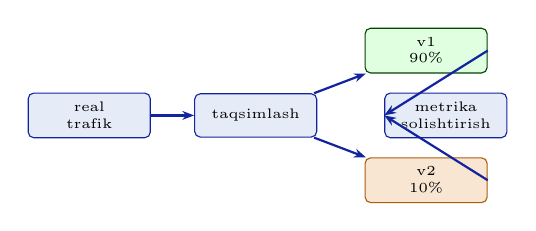
\begin{tikzpicture}[
        n/.style={draw=cnublue,fill=cnubluebg,rounded corners=2pt,
                  minimum width=1.55cm,minimum height=0.55cm,
                  align=center,font=\tiny},
        g/.style={draw=deepgreen!60!black,fill=green!12,rounded corners=2pt,
                  minimum width=1.55cm,minimum height=0.55cm,
                  align=center,font=\tiny},
        r/.style={draw=cwarn!80!black,fill=cwarn!18,rounded corners=2pt,
                  minimum width=1.55cm,minimum height=0.55cm,
                  align=center,font=\tiny},
        a/.style={-{Stealth[length=1.5mm]},thick,cnublue}
      ]
        \node[n] (u) {real\\trafik};
        \node[n, right=0.55cm of u] (split) {taqsimlash};
        \node[g, above right=0.25cm and 0.6cm of split] (v1) {v1\\90\%};
        \node[r, below right=0.25cm and 0.6cm of split] (v2) {v2\\10\%};
        \node[n, right=0.85cm of split] (m) {metrika\\solishtirish};

        \draw[a] (u)--(split);
        \draw[a] (split)--(v1);
        \draw[a] (split)--(v2);
        \draw[a] (v1.east)--(m.west);
        \draw[a] (v2.east)--(m.west);
      \end{tikzpicture}

      \vspace{4pt}

      \begin{tcolorbox}[okbox,top=2pt,bottom=2pt]
        \footnotesize
        Agar v2 asosiy metrikalarda yaxshi, xavfsizlik metrikalarida esa
        yomonlashmagan bo\uzq{}lsa, trafik bosqichma-bosqich oshiriladi;
        aks holda rollback qilinadi.
      \end{tcolorbox}
    \end{column}
  \end{columns}
\end{frame}

\begin{frame}[fragile]{Ilova S2: smoke test --- deploydan keyingi tezkor tekshiruv}
  \small

  Deploydan keyin xizmat haqiqatan ishga tushganini minimal so\uzq{}rov bilan
  tekshiramiz:

\begin{lstlisting}[language=bash,basicstyle=\ttfamily\scriptsize]
curl -s -X POST http://localhost:8000/predict \
  -H "Content-Type: application/json" \
  -d '{"text": "mahsulot juda yaxshi"}'

# kutilgan javob:
# {"label": "ijobiy", "confidence": 0.92}
\end{lstlisting}

  \vspace{3pt}

  \begin{columns}[T,totalwidth=\textwidth]
    \begin{column}{0.52\textwidth}
      \begin{tcolorbox}[defbox,top=2pt,bottom=2pt,left=4pt,right=4pt]
        \footnotesize
        \textbf{Smoke test} --- tizimning eng muhim yo\uzq{}li ishlayotganini
        tekshiruvchi \textbf{minimal nazorat sinovi}.
      \end{tcolorbox}
    \end{column}

    \begin{column}{0.45\textwidth}
      \begin{tcolorbox}[okbox,top=2pt,bottom=2pt,left=4pt,right=4pt]
        \footnotesize
        \textbf{Tekshiramiz:}
        endpoint javob berdimi, JSON format to\uzq{}rimi,
        \texttt{label} va \texttt{confidence} qaytdimi.
      \end{tcolorbox}
    \end{column}
  \end{columns}

  \vspace{3pt}

  {\scriptsize
  CI/CD jarayonida bunday test deploydan keyin avtomatik bajariladi.
  Agar smoke test o\uzq{}tmasa, yangi versiya production uchun xavfli deb qaraladi.
  }
\end{frame}

\end{document}
